% HISTORICAL REPORT: previous dataset. Current final-data results: reports/final_dataset/README.md.
% Standalone editable source. Compile with pdfLaTeX or LuaLaTeX.
% All table values and plot coordinates are embedded. No additional files, API keys or downloads are required.
% Main section followed by an empirical appendix. Results verified against the local source on 12 October 2026.
% Canonical analytical source: VAR_QTFE.ipynb and reports/var_har_notebook/generated.
\documentclass[11pt,letterpaper]{article}
\usepackage[margin=1in]{geometry}
\usepackage[T1]{fontenc}
\usepackage{lmodern}
\usepackage{amsmath,amssymb,booktabs,array,tabularx,float,caption}
\usepackage{pgfplots}
\usepgfplotslibrary{groupplots,fillbetween}
\usepackage[hidelinks]{hyperref}
\pgfplotsset{compat=1.18}
\definecolor{reportblue}{RGB}{35,80,125}
\definecolor{reportorange}{RGB}{185,95,35}
\definecolor{reportgreen}{RGB}{45,120,95}
\setlength{\parindent}{0pt}
\setlength{\parskip}{5pt}
\setlength{\tabcolsep}{5pt}
\renewcommand{\arraystretch}{1.15}
\captionsetup{font=small,labelfont=bf,justification=raggedright,singlelinecheck=false,position=top,skip=5pt}
\hypersetup{pdftitle={LVAR analysis of equity realised variance},pdfauthor={}}
\newcommand{\sourcefile}[1]{\texttt{\small #1}}
\newcommand{\appendixpage}[2]{\clearpage\section*{#1}\label{#2}}
\begin{document}
{\Large\bfseries LVAR analysis of equity realised variance\par}
{\small Empirical methodology and results\hfill 12 October 2026\par}
\vspace{6pt}

\begin{quote}
\textbf{Historical dataset report.} The tables and figures below describe the
previous data version. HAR and VAR were rerun on the final wide CSV on
13 October 2026; the current evaluation has 783 targets, rather than 802.
Use \texttt{reports/final\_dataset/README.md} and the executed root notebooks
for the updated results. This report's embedded numerical results have not been
rewritten for the final dataset.
\end{quote}

\section*{Data construction and common evaluation sample}
We examine whether commodity variance histories improve forecasts of equity realised
variance beyond equity history and negative equity-return information. Downside inputs
reduce forecast MSE by about 9\%, while oil and gold provide little incremental
benefit. This distinction matters for risk forecasting: a multivariate model can
improve on persistence because it captures equity dynamics, even when additional
markets do not improve a matched equity benchmark.

We use the VOLARE daily five-minute realised variance measure, RV5, for S\&P 500
equity futures (ES), crude oil (CL), gold (GC), corn (C) and natural gas (NG)
\cite{volare}. The target is ES log RV5. Each futures variance enters in natural
logarithms; no square root or annualisation is applied. Realised volatility is the
square root of realised variance, so the reported target and loss units should be
described as variance rather than volatility. The main system contains ES, oil and
gold; corn and gas provide extensions.

We begin with observations from 2011 and retain a common calendar across all five
markets, including for models that use fewer markets. This reproduces the commodity
preparation used by the asymmetric HAR comparison. Asset-specific close returns and
five-/22-observation variance averages are constructed on source dates before
matching markets. Complete cases are then retained without filling missing RV5.
The downside-return windows are constructed after this matching step. The common
design reserves the initial 21 retained origins for the longest downside window
and omits the final origin without a next target.

\begin{table}[H]
\centering\caption{Common sample and evaluation period}\label{tab:sample}
\small\begin{tabular}{p{2.5in}p{2.5in}r}\toprule
Sample & Dates & Observations\\\midrule
Prepared five-market panel & 1 Feb 2011 to 31 Aug 2026 & 3,989\\
Initial fitted training targets & 3 Mar 2011 to 12 Jul 2023 & 3,165\\
Evaluation targets & 13 Jul 2023 to 31 Aug 2026 & 802\\
All common regression targets & 3 Mar 2011 to 31 Aug 2026 & 3,967\\\bottomrule
\end{tabular}\end{table}
{\footnotesize The initial fitted split is 79.78\% training and 20.22\% evaluation.
Counts refer to target outcomes after common feature construction; the prepared panel
and initial stationarity sample are larger.\par}

The training cutoff remains fixed at 12 July 2023. Every model scores the same 802
targets, preventing a change in calendar from driving model rankings. A one-step
forecast targets the next retained common observation, which need not be the next
original ES observation. Eight evaluation transitions skip an observed ES date;
the target remains the later date's daily RV5. Treasury inputs and calendar dummy
controls do not enter this specification. The newer HAR yield join is audited
separately and must not determine the commodity comparison calendar.

\clearpage
\section*{VAR methodology and forecast results}
We estimate VARs with an intercept and individual lags of the included markets'
log variances. We call the leverage-augmented versions \textbf{LVAR}. They include
three predetermined ES downside
inputs: the negative parts of the latest decimal return and the five-/22-observation
mean returns. The negative part is taken after averaging. These controls enter every
equation, giving a linear VAR with exogenous downside inputs, rather than a regime
switching model. Leverage here refers to the asymmetric association between negative
equity returns and variance, not borrowing. LVAR's variance-lag coefficients do not
switch across regimes. Appendix~B1 gives the exact definition.

The matched benchmark is an equity-only AR with the same lag order, calendar and
downside inputs. The plain versions omit downside controls from both AR and VAR.
This separates the contribution of commodity histories from the contribution of
negative equity-return information. We estimate each equation by OLS. Bartlett
HAC(22) standard errors are used for coefficient screens; this changes inference,
not the OLS coefficients or forecasts.

Lag selection uses the plain five-market system and only initial training outcomes.
Among orders 1--20, BIC selects five and AIC selects ten. We retain five as the main
order and ten as a fixed sensitivity. Both orders use the same training outcomes.
Before every forecast, coefficients are re-estimated with an expanding history:
the first fit uses 3,165 known outcomes and the last uses 3,966. Forecast errors concern
only the ES equation. MSE is the primary loss; RMSE, MAE and variance-scale QLIKE
provide supporting checks. All primary and sensitivity forecasts use zero fallbacks.

\begin{table}[H]
\centering
\caption{Primary forecast accuracy with five lags}\label{tab:primary}
\small
\begin{tabular}{p{3.85in}rr}
\toprule
Model & MSE & Gain (\%) \\
\midrule
\multicolumn{3}{l}{\textit{Variance history only with the plain AR benchmark}} \\
Equity AR & 0.409476 & +0.000 \\
Corn VAR & 0.411058 & -0.386 \\
Gold VAR & 0.412495 & -0.737 \\
Oil and gold VAR & 0.413082 & -0.881 \\
All four commodity VAR & 0.412453 & -0.727 \\
\addlinespace\multicolumn{3}{l}{\textit{Downside information with the downside AR benchmark}} \\
Equity AR with downside & 0.371498 & +0.000 \\
Corn LVAR & 0.373076 & -0.425 \\
Gold LVAR & 0.374554 & -0.823 \\
Oil and gold LVAR & 0.374172 & -0.720 \\
Gas LVAR & 0.370016 & +0.399 \\
Oil gold and gas LVAR & 0.371957 & -0.123 \\
All four LVAR & 0.372801 & -0.351 \\
\bottomrule
\end{tabular}
\end{table}
{\footnotesize All models score the same 802 next-observation ES log RV5 targets. Gain equals $100(1-\mathrm{MSE}_{model}/\mathrm{MSE}_{benchmark})$; positive values favour the model. Benchmarks differ between the two explicitly labelled groups. The persistence MSE is 0.500185.\par}


Adding downside inputs lowers the main oil--gold system's MSE from 0.413082 to
0.374172, a 9.42\% reduction. The equity-only reduction is similar at 9.27\%.
However, the oil--gold LVAR has 0.72\% higher MSE than the matched downside
AR. Adding all four commodities raises MSE by 0.35\%; gas alone lowers it by 0.40\%.
The useful additional information therefore comes mainly from equity downside
signals. The small commodity differences do not establish reliable forecast gains.

Gold-only VAR and LVAR were added as exploratory comparisons on 12 October 2026.
They include ES and gold, with the same five lags, calendar and expanding protocol.
Their MSEs exceed the matching equity-only benchmarks by 0.74\%
and 0.82\%, respectively. They do not improve forecasting in this evaluation.

Corn-only VAR and LVAR were also added as exploratory comparisons on 12 October
2026, using ES and corn with the same five lags, common dates and expanding protocol.
Their MSEs exceed the matching equity-only benchmarks by 0.39\%
and 0.42\%, respectively. No fallback forecasts were needed.

\clearpage
\section*{Sensitivity evidence and interpretation}
Longer variance histories improve the observed MSEs. At ten lags, the oil--gold
LVAR scores 0.368497 rather than 0.374172, a 1.52\% reduction. The equity
downside AR also improves, to 0.365892, so the oil--gold system remains about 0.71\%
worse. The all-four VAR is almost tied with the AR(10), while gas has a small
0.58\% point advantage. All eight tested plain/downside lag comparisons favour
ten lags by MSE. These inspected scores support a lag sensitivity, not a claim
that ten is an optimal order or a reason to replace the initial BIC choice.

The matched equity-only asymmetric HAR has MSE 0.362110. Its advantage over the
downside AR is 2.53\% at five lags and about 1.03\% at ten. HAR represents variance
memory through daily, weekly and monthly averages \cite{corsi}; VAR uses individual
lags. The comparison shares outcomes, downside controls and training dates, but
the two memory representations differ. The matched HAR forecasts are independently
reproduced from the group's current HAR function. Its separate yield-joined
standalone scores are not part of this ranking.

Data sensitivities preserve the main finding. Omitting suspect training windows,
using open-to-close ES downside returns, or replacing RV5 predictors and outcomes
with realised kernel estimates leaves the equity downside gain near 9--10\%.
Oil and gold do not improve the matching downside benchmark in any of these
scenarios. The small all-four gain changes sign under RK, which shows sensitivity
to the variance proxy. RK and RV5 losses measure different outcomes and should
not be ranked by their raw MSEs. On a retrospective 725-target subset excluding
flag-exposed windows, gas's gain falls from 0.40\% to 0.12\%.

Descriptive paired-loss intervals also qualify the commodity differences.
The 95\% interval for oil and gold is [\(-2.02\), \(+0.66\)]\% and for gas is
[\(-1.22\), \(+2.01\)]\%. Both allow gains and losses. These fixed-forecast block
resamples are exploratory and do not constitute a formal nested-model test or a
correction for prior model selection. Appendix~C2 reports the
definitions and uncertainty calculations.

The initial-training five-market extension's generalized IRFs provide a separate
description of fitted dynamics \cite{pesaran}. At horizon five, one residual-standard-
deviation commodity log-variance innovation is associated with implied ES variance
responses of 8.31\% for oil, 3.71\% for corn, 8.55\% for gold and 5.24\% for gas.
Responses generally dissipate, although gas is not monotonic. Controls follow the
same path in the shocked and baseline systems. These conditional responses and
their exploratory pointwise bands describe fitted associations; they do not
identify causal commodity shocks or demonstrate additional forecast value.

Our conclusion is specific to this target, sample and forecasting protocol.
ADF and KPSS give conflicting stationarity evidence, and initial residual screens
show remaining serial dependence. Futures returns are not adjusted for contract
rolls. Daily aggregates cannot validate flagged quotes or resolve exact session
labels and estimate publication times. The evaluation period has already been
examined, so the reported comparisons remain exploratory. Within these limits,
negative equity-return information improves forecasts, whereas commodity histories
provide little consistent incremental benefit beyond a matching equity model.

\clearpage
\appendix
\setcounter{table}{0}\renewcommand{\thetable}{A\arabic{table}}
\setcounter{figure}{0}\renewcommand{\thefigure}{A\arabic{figure}}
\section*{Appendix A Data definitions and forecast timing}\label{app:data}
The appendix documents the common inputs and evidence behind the main comparison.
The source is the local VOLARE export ending on 31 August 2026. The 2011 restriction
provides compatibility with the HAR analysis; it does not eliminate later calendar,
quote or rollover concerns. The raw export and review ledger are preserved.

\begin{table}[H]
\centering
\caption{Variables in the commodity comparison}\label{tab:definitions}
\small
\begin{tabular}{p{0.9in}p{2.6in}p{2.35in}}
\toprule
Variable & Meaning & Input transformation \\
\midrule
ES & S\&P 500 equity futures & $\log(\mathrm{RV5})$ \\
CL & Crude oil futures & $\log(\mathrm{RV5})$ \\
GC & Gold futures & $\log(\mathrm{RV5})$ \\
C & Corn futures & $\log(\mathrm{RV5})$ \\
NG & Natural gas futures & $\log(\mathrm{RV5})$ \\
$d^{(1)},d^{(5)},d^{(22)}$ & ES downside return controls & Negative part of the mean decimal return \\
\bottomrule
\end{tabular}
\end{table}
{\footnotesize VOLARE provides the RV5 and close-price inputs. Returns are calculated on each asset\textquotesingle s source dates before matching markets. Downside windows are calculated over retained common rows. RV5 is variance; no square root or annualisation is applied.\par}

\begin{table}[H]
\centering
\caption{Descriptive statistics of the common log RV5 outcomes}\label{tab:stats}
\footnotesize
\begin{tabular}{llrrrrr}
\toprule
Sample & Market & Mean & SD & Median & Min & Max \\
\midrule
Training & ES & -9.781 & 1.072 & -9.877 & -13.874 & -5.055 \\
Training & CL & -8.032 & 0.959 & -8.074 & -11.423 & -0.696 \\
Training & GC & -9.626 & 0.745 & -9.681 & -12.123 & -6.179 \\
Training & C & -8.732 & 0.857 & -8.783 & -11.943 & -4.530 \\
Training & NG & -7.417 & 0.868 & -7.534 & -10.254 & -2.707 \\
Evaluation & ES & -9.923 & 0.879 & -9.986 & -12.834 & -5.285 \\
Evaluation & CL & -7.925 & 0.815 & -8.080 & -9.975 & -3.565 \\
Evaluation & GC & -9.321 & 0.855 & -9.389 & -11.571 & -5.510 \\
Evaluation & C & -8.935 & 0.714 & -8.947 & -11.926 & -5.579 \\
Evaluation & NG & -6.845 & 0.598 & -6.928 & -8.177 & -3.388 \\
\bottomrule
\end{tabular}
\end{table}
{\footnotesize Training $n=3{,}165$; evaluation $n=802$. Statistics use the dated target outcomes, not the larger 3,187-row panel used for initial stationarity checks. Evaluation statistics are descriptive and do not select models.\par}

\begin{table}[H]
\centering
\caption{Examples of the forecast information set}\label{tab:timing}
\footnotesize
\begin{tabular}{llrr}
\toprule
Target date & Information through & Training rows & Skipped ES dates \\
\midrule
13 Jul 2023 & 12 Jul 2023 & 3,165 & 0 \\
24 Nov 2023 & 22 Nov 2023 & 3,260 & 1 \\
05 Jul 2024 & 03 Jul 2024 & 3,416 & 1 \\
31 Aug 2026 & 28 Aug 2026 & 3,966 & 0 \\
\bottomrule
\end{tabular}
\end{table}
{\footnotesize Skipped dates are observed original ES dates strictly between the forecast origin and target; ordinary weekends do not count. Eight of the 802 transitions skip at least one such ES date. The target remains that date\textquotesingle s daily RV5, not variance accumulated across the gap.\par}


\appendixpage{Appendix B1 Model definition and lag selection}{app:specification}
\setcounter{table}{0}\renewcommand{\thetable}{B\arabic{table}}
\setcounter{figure}{0}\renewcommand{\thefigure}{B\arabic{figure}}
Let $y_t$ contain the log RV5 values for ES and the commodities in a particular
system, with $t$ indexing retained common observations. The forecast equation is
\begin{equation}
y_{t+1}=c+\sum_{j=1}^{p} A_j y_{t+1-j}+\Gamma d_t+u_{t+1}.
\label{eq:var}
\end{equation}
At origin $t$, lag one is the latest observed $y_t$. The three downside inputs are
\begin{equation}
d_t=\bigl(d_t^{(1)},d_t^{(5)},d_t^{(22)}\bigr)',\qquad
d_t^{(k)}=-\min\!\left\{\frac{1}{k}\sum_{i=0}^{k-1}r_{t-i},0\right\}.
\label{eq:downside}
\end{equation}
Here $r_t$ is the decimal ES close log return constructed on source dates. Stored
percentage returns are divided by 100. A negative mean becomes a positive downside
magnitude; a nonnegative mean becomes zero. This is the negative part of a mean,
not the mean of daily negative parts. The plain model sets $\Gamma=0$. The equity-only
system is the corresponding AR. No future return is supplied to a forecast.

\begin{figure}[H]
\centering
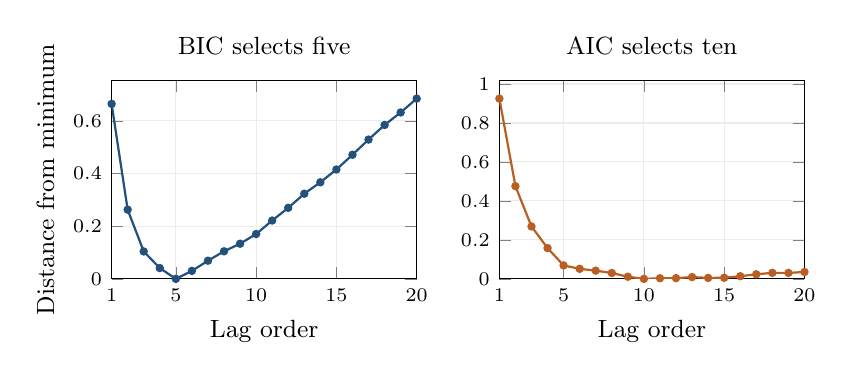
\begin{tikzpicture}
\begin{groupplot}[group style={group size=2 by 1,horizontal sep=1.05cm},width=0.45\textwidth,height=4.1cm,
 xlabel={Lag order},ylabel={Distance from minimum},xmin=1,xmax=20,xtick={1,5,10,15,20},ymin=0,
 tick label style={font=\scriptsize},label style={font=\small},title style={font=\small},grid=major,grid style={gray!15}]
\nextgroupplot[title={BIC selects five}]
\addplot[reportblue,thick,mark=*,mark size=1.1pt] coordinates {(1,0.66435028) (2,0.26284428) (3,0.10412319) (4,0.04120131) (5,0.00000000) (6,0.03045497) (7,0.06893269) (8,0.10476661) (9,0.13351605) (10,0.17029664) (11,0.22156609) (12,0.26981451) (13,0.32325270) (14,0.36677029) (15,0.41528418) (16,0.47126640) (17,0.52892773) (18,0.58423423) (19,0.63177464) (20,0.68442397)};
\nextgroupplot[title={AIC selects ten},ylabel={}]
\addplot[reportorange,thick,mark=*,mark size=1.1pt] coordinates {(1,0.92485281) (2,0.47548023) (3,0.26889257) (4,0.15810412) (5,0.06903623) (6,0.05162463) (7,0.04223577) (8,0.03020312) (9,0.01108598) (10,0.00000000) (11,0.00340288) (12,0.00378472) (13,0.00935633) (14,0.00500736) (15,0.00565467) (16,0.01377031) (17,0.02356507) (18,0.03100500) (19,0.03067883) (20,0.03546159)};
\end{groupplot}
\end{tikzpicture}
\caption{Initial training information criteria for the plain five-market VAR}\label{fig:lags}
\end{figure}
{\footnotesize Orders 1--20 use the same 3,165 training outcomes and an intercept. Each criterion is shown relative to its own minimum. No downside or calendar controls enter this lag-selection system. Source: initial\_lag\_selection.csv.\par}

\begin{table}[H]
\centering
\caption{Coefficients in the downside specifications}\label{tab:parameters}
\small
\begin{tabular}{p{2.3in}rrrr}
\toprule
System & ES at 5 & System at 5 & ES at 10 & System at 10 \\
\midrule
Equity only & 9 & 9 & 14 & 14 \\
Equity and gas & 14 & 28 & 24 & 48 \\
Equity oil and gold & 19 & 57 & 34 & 102 \\
Equity and all four commodities & 29 & 145 & 54 & 270 \\
\bottomrule
\end{tabular}
\end{table}
{\footnotesize Counts include one intercept and three downside coefficients per equation. The plain counterparts omit the three downside coefficients. The matched AR also uses the common lag order; its lag length is not selected independently.\par}


Daily-only commodity restrictions set commodity lag coefficients after lag one
to zero in every equation. ES retains all $p$ variance lags and all three downside
windows. HAR's daily/weekly/monthly averages and these VAR lags are distinct
representations of memory. Lag selection is shared across systems to keep the
commodity comparison focused on information sets rather than different lag choices.

\appendixpage{Appendix B2 Stationarity and residual evidence}{app:diagnostics}
\begin{table}[H]
\centering
\caption{Stationarity screens using initial history}\label{tab:stationarity}
\small
\begin{tabular}{lrrrr}
\toprule
Market & Observations & ADF statistic & ADF p & KPSS statistic \\
\midrule
ES & 3,187 & -5.669 & 9.03e-07 & 0.768 \\
CL & 3,187 & -4.158 & 0.000776 & 1.789 \\
C & 3,187 & -5.478 & 2.32e-06 & 0.751 \\
GC & 3,187 & -4.903 & 3.44e-05 & 0.877 \\
NG & 3,187 & -3.659 & 0.00473 & 2.468 \\
\bottomrule
\end{tabular}
\end{table}
{\footnotesize ADF includes an intercept and selects difference lags by AIC with the statsmodels default maximum. KPSS tests level stationarity with its automatic bandwidth; every KPSS p-value is below the 0.01 tabulation boundary. Both use the prepared panel through 12 July 2023, including the extra rows used to form model inputs.\par}

ADF rejects a unit root, while KPSS rejects level stationarity for all five inputs.
We retain the level-in-log specification for the stated forecast comparison, but
do not regard these screens as proof of stationarity or a diagnosed structural break.

\begin{table}[H]
\centering
\caption{Initial training equity residual diagnostics}\label{tab:diagnostics}
\small
\begin{tabular}{p{2.5in}rrr}
\toprule
Model & Ljung--Box p & ARCH p & Largest root \\
\midrule
Equity AR with downside & 1.6e-10 & 0.092 & 0.917 \\
Oil and gold LVAR & 6.21e-06 & 0.080 & 0.967 \\
All four LVAR & 0.000278 & 0.099 & 0.979 \\
\bottomrule
\end{tabular}
\end{table}
{\footnotesize All rows use 3,165 initial training targets. Ljung--Box uses 30 lags and no degrees-of-freedom adjustment; it is an ES residual screen, not a calibrated multivariate VAR whiteness test. ARCH uses five lags. Roots refer to the conditional variance dynamics.\par}

The largest conditional roots are below one. This describes the fitted variance
lag dynamics while holding the return-control process outside the system. It does
not validate the full model. Ljung--Box screens indicate remaining dependence;
the five-lag ARCH screens above 0.05 do not establish constant error variance.

\begin{table}[H]
\centering
\caption{Joint commodity coefficient screens}\label{tab:joint}
\footnotesize
\begin{tabular}{llrrr}
\toprule
System & Coefficients tested & Number & Wald & HAC p \\
\midrule
Oil and gold & Oil & 5 & 21.384 & 0.000685 \\
Oil and gold & Gold & 5 & 15.362 & 0.00892 \\
Oil and gold & All included commodities & 10 & 38.047 & 3.72e-05 \\
All four & Natural gas & 5 & 29.769 & 1.64e-05 \\
All four & Corn & 5 & 4.824 & 0.438 \\
All four & All included commodities & 20 & 85.585 & 4.34e-10 \\
\bottomrule
\end{tabular}
\end{table}
{\footnotesize Initial training ES equations; Bartlett HAC with 22 lags and no small-sample correction. Tests condition on ES history and matching downside inputs. P-values are exploratory and unadjusted for multiple comparisons. They test fitted conditional associations, not causal effects or forecast-loss superiority.\par}

Oil and gold are jointly associated with ES in the initial fitted equation, even
though they do not improve the matched forecast benchmark. Fitted coefficient
screens and forecasts on later outcomes answer different questions.

For the full-sample ES equation, the oil--gold LVAR has $R^2=0.7231$,
compared with 0.7208 for the downside AR. Both fits include all 3,967 outcomes,
including evaluation observations. The slightly better historical fit does not
establish a forecasting gain.

\appendixpage{Appendix B3 Conditional impulse response curves}{app:irfs}
We estimate the five-market LVAR(5) on the 3,165 initial training outcomes,
ending 12 July 2023. For innovation covariance $\Sigma$ and moving-average
coefficient matrix $\Phi_h$, the generalized log response to market $j$ is
\begin{equation}
g_j(h)=\frac{\Phi_h\Sigma e_j}{\sqrt{\Sigma_{jj}}},
\qquad \Phi_0=I.
\end{equation}
This is invariant to market ordering \cite{pesaran}. Correlated innovations
generate contemporaneous co-movement at horizon zero. Downside controls follow an
identical fixed path in shocked and baseline forecasts; future-return feedback is
not simulated. For ES log response $a$, the implied variance response is
$100(e^a-1)$\%, and the implied volatility response is $100(e^{a/2}-1)$\%.

\begin{figure}[H]
\centering
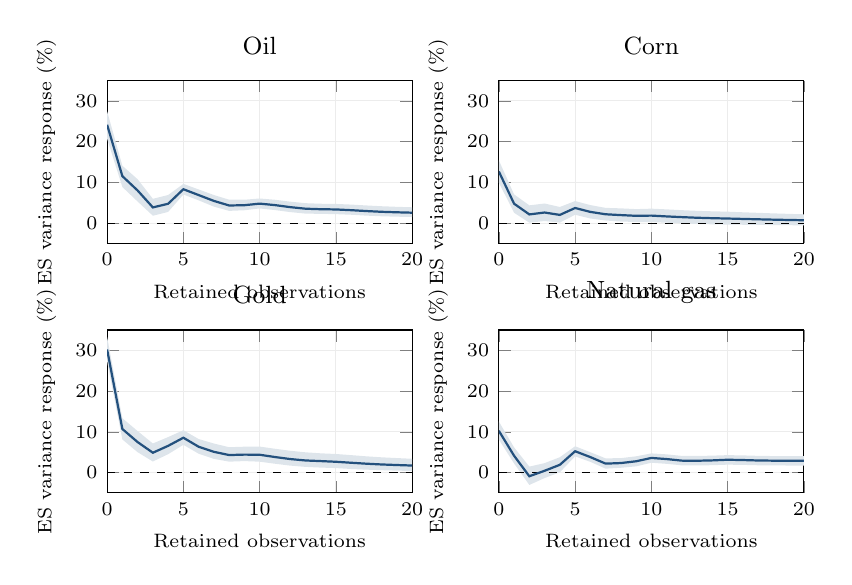
\begin{tikzpicture}
\begin{groupplot}[group style={group size=2 by 2,horizontal sep=1.1cm,vertical sep=1.1cm},
 width=0.45\textwidth,height=3.65cm,xmin=0,xmax=20,ymin=-5,ymax=35,
 xlabel={Retained observations},ylabel={ES variance response (\%)},xtick={0,5,10,15,20},
 tick label style={font=\scriptsize},label style={font=\scriptsize},title style={font=\small},
 grid=major,grid style={gray!15}]
\nextgroupplot[title={Oil}]
\addplot[draw=none,name path=cllower] coordinates {(0,20.71638737) (1,8.85814762) (2,5.29098653) (3,1.80567030) (4,2.74445039) (5,7.01259292) (6,5.58134807) (7,4.03686559) (8,2.99928532) (9,3.15129870) (10,3.58825495) (11,3.19633454) (12,2.69838153) (13,2.32943141) (14,2.26088370) (15,2.19502332) (16,2.04561407) (17,1.82858946) (18,1.66627700) (19,1.56824461) (20,1.48548918)};
\addplot[draw=none,name path=clupper] coordinates {(0,27.45744459) (1,14.07970467) (2,10.76562423) (3,5.95892807) (4,6.89811336) (5,9.62581119) (6,8.26031955) (7,6.88727190) (8,5.74392741) (9,5.73085498) (10,6.04188746) (11,5.72646187) (12,5.26073031) (13,4.88726657) (14,4.75001542) (15,4.70145468) (16,4.54074679) (17,4.32726668) (18,4.13730631) (19,3.99007452) (20,3.87698343)};
\addplot[reportblue!15,draw=none] fill between[of=cllower and clupper];
\addplot[black,dashed,thin] coordinates {(0,0) (20,0)};
\addplot[reportblue,thick] coordinates {(0,24.14528025) (1,11.52733156) (2,7.99854764) (3,3.84746962) (4,4.74267723) (5,8.31360558) (6,6.87886388) (7,5.44079285) (8,4.32107914) (9,4.38947594) (10,4.77862165) (11,4.41572538) (12,3.91718624) (13,3.53127571) (14,3.40632570) (15,3.34757187) (16,3.16741354) (17,2.95291940) (18,2.76958510) (19,2.64862719) (20,2.54974312)};
\nextgroupplot[title={Corn}]
\addplot[draw=none,name path=clower] coordinates {(0,9.96483805) (1,2.53175684) (2,0.09519091) (3,0.50569194) (4,0.12042132) (5,2.03761181) (6,1.12705730) (7,0.63037606) (8,0.37531396) (9,0.27062397) (10,0.23080835) (11,0.09041703) (12,-0.07959548) (13,-0.21051107) (14,-0.30742071) (15,-0.36943073) (16,-0.41233007) (17,-0.44272743) (18,-0.49059231) (19,-0.52568970) (20,-0.55631945)};
\addplot[draw=none,name path=cupper] coordinates {(0,15.42053849) (1,7.04568638) (2,4.35432019) (3,4.80921357) (4,3.95324806) (5,5.41051488) (6,4.41957147) (7,3.73461660) (8,3.61403914) (9,3.43107759) (10,3.54140347) (11,3.36664293) (12,3.16873596) (13,3.00566925) (14,2.88923888) (15,2.79805214) (16,2.65169507) (17,2.51621618) (18,2.38064482) (19,2.26332593) (20,2.15655061)};
\addplot[reportblue!15,draw=none] fill between[of=clower and cupper];
\addplot[black,dashed,thin] coordinates {(0,0) (20,0)};
\addplot[reportblue,thick] coordinates {(0,12.67931733) (1,4.76157005) (2,2.12762586) (3,2.59131701) (4,2.00778571) (5,3.70502807) (6,2.74549619) (7,2.16429131) (8,1.95972774) (9,1.78333547) (10,1.83534885) (11,1.63514312) (12,1.45975798) (13,1.30818529) (14,1.19949494) (15,1.11522489) (16,1.01896843) (17,0.92745449) (18,0.83843888) (19,0.76458264) (20,0.69814678)};
\nextgroupplot[title={Gold}]
\addplot[draw=none,name path=gclower] coordinates {(0,27.34152310) (1,8.13126762) (2,5.00068298) (3,2.71423158) (4,4.50906421) (5,6.81528114) (6,4.62641605) (7,3.35705895) (8,2.67610559) (9,2.81565781) (10,2.67005661) (11,2.16618051) (12,1.70475792) (13,1.39491232) (14,1.22111971) (15,1.09852022) (16,0.87439317) (17,0.70977594) (18,0.57971318) (19,0.47267123) (20,0.38336842)};
\addplot[draw=none,name path=gcupper] coordinates {(0,33.28034207) (1,13.35052569) (2,10.18579194) (3,7.14039414) (4,8.71397695) (5,10.40028745) (6,8.23360502) (7,7.13097303) (8,6.22408220) (9,6.35240882) (10,6.37666886) (11,5.84689356) (12,5.35430730) (13,4.97194107) (14,4.72392907) (15,4.56108975) (16,4.27853001) (17,3.98701111) (18,3.74077183) (19,3.55988261) (20,3.38158275)};
\addplot[reportblue!15,draw=none] fill between[of=gclower and gcupper];
\addplot[black,dashed,thin] coordinates {(0,0) (20,0)};
\addplot[reportblue,thick] coordinates {(0,30.22019264) (1,10.69960072) (2,7.48420653) (3,4.87078939) (4,6.55962902) (5,8.55482500) (6,6.33805590) (7,5.09241900) (8,4.29952311) (9,4.40682285) (10,4.37347547) (11,3.81498997) (12,3.31803043) (13,2.96989707) (14,2.81547056) (15,2.65090432) (16,2.40790599) (17,2.17430052) (18,1.98614103) (19,1.84846988) (20,1.72077635)};
\nextgroupplot[title={Natural gas}]
\addplot[draw=none,name path=nglower] coordinates {(0,8.11637760) (1,2.23374572) (2,-3.04251224) (3,-1.35600149) (4,0.06853311) (5,3.97840614) (6,2.62552410) (7,0.95530091) (8,1.17638972) (9,1.52187657) (10,2.40789227) (11,2.14269020) (12,1.76661509) (13,1.74019321) (14,1.80925422) (15,1.93734027) (16,1.88212547) (17,1.78638509) (18,1.75296317) (19,1.72856036) (20,1.73208116)};
\addplot[draw=none,name path=ngupper] coordinates {(0,12.54697771) (1,6.18411390) (2,1.46159277) (3,2.31824027) (4,3.76913601) (5,6.45675692) (6,5.00019473) (7,3.48758127) (8,3.54561738) (9,3.98884017) (10,4.70949358) (11,4.47337013) (12,4.09007082) (13,4.07363070) (14,4.15501207) (15,4.27891669) (16,4.21336722) (17,4.10556275) (18,4.05318545) (19,4.02964227) (20,4.02231262)};
\addplot[reportblue!15,draw=none] fill between[of=nglower and ngupper];
\addplot[black,dashed,thin] coordinates {(0,0) (20,0)};
\addplot[reportblue,thick] coordinates {(0,10.25657761) (1,4.12903973) (2,-0.90612531) (3,0.43705958) (4,1.90454953) (5,5.23809415) (6,3.79667369) (7,2.19295818) (8,2.33397675) (9,2.77052502) (10,3.58939211) (11,3.31430575) (12,2.92716444) (13,2.90228010) (14,2.98940977) (15,3.14701231) (16,3.07378847) (17,2.96313599) (18,2.92002762) (19,2.90895283) (20,2.90950105)};

\end{groupplot}
\end{tikzpicture}
\caption{Conditional generalized responses to commodity log variance innovations}\label{fig:irfs}
\end{figure}
{\footnotesize Initial training five-market LVAR(5), not the main three-market system. Curves are percentage changes in the implied ES variance path. Shading is an exploratory 95\% pointwise parameter band; axes are shared. Each innovation is one market-specific residual standard deviation. Source: training\_generalized\_irfs.csv.\par}

\begin{table}[H]
\centering
\caption{Selected implied ES variance responses in percent}\label{tab:irfs}
\footnotesize
\begin{tabular}{lrrrr}
\toprule
Innovation & Horizon 1 & Horizon 5 & Horizon 20 & Horizon 20 band \\
\midrule
Oil & +11.53 & +8.31 & +2.55 & [+1.49, +3.88] \\
Corn & +4.76 & +3.71 & +0.70 & [-0.56, +2.16] \\
Gold & +10.70 & +8.55 & +1.72 & [+0.38, +3.38] \\
Natural gas & +4.13 & +5.24 & +2.91 & [+1.73, +4.02] \\
\bottomrule
\end{tabular}
\end{table}
{\footnotesize Horizons count retained common observations. Horizon zero is contemporaneous co-movement. Responses are relative to the unshocked path, not equity price returns or causal effects.\par}


Bands jointly simulate OLS coefficients and innovation covariance using Bartlett
HAC(22), including their cross covariance. All 2,000 draws are stable and positive
definite at seed 20261005; the point root is 0.978582. The 95\% bands are pointwise,
asymptotic and exploratory, conditional on admissible draws. They are neither
prediction bands nor causal uncertainty intervals. Back-transformation describes
the log-model path, not a separately estimated arithmetic conditional-variance mean.

\appendixpage{Appendix C1 Detailed forecast accuracy}{app:accuracy}
\setcounter{table}{0}\renewcommand{\thetable}{C\arabic{table}}
\setcounter{figure}{0}\renewcommand{\thefigure}{C\arabic{figure}}
\begin{table}[H]
\centering
\caption{Detailed primary VAR forecast comparison at five lags}\label{tab:completeaccuracy}
\footnotesize
\begin{tabular}{p{2.8in}rrrr}
\toprule
Model & MSE & RMSE & MAE & Gain (\%) \\
\midrule
Equity AR & 0.409476 & 0.639903 & 0.487944 & +0.000 \\
Corn VAR & 0.411058 & 0.641138 & 0.489017 & -0.386 \\
Gold VAR & 0.412495 & 0.642257 & 0.488358 & -0.737 \\
Oil and gold VAR & 0.413082 & 0.642715 & 0.488721 & -0.881 \\
All four VAR & 0.412453 & 0.642225 & 0.488647 & -0.727 \\
\addlinespace
Equity AR + downside & 0.371498 & 0.609507 & 0.465084 & +0.000 \\
Corn LVAR & 0.373076 & 0.610799 & 0.466739 & -0.425 \\
Gold LVAR & 0.374554 & 0.612008 & 0.465820 & -0.823 \\
Oil and gold LVAR & 0.374172 & 0.611696 & 0.465399 & -0.720 \\
Gas LVAR & 0.370016 & 0.608290 & 0.464493 & +0.399 \\
Oil gold and gas LVAR & 0.371957 & 0.609883 & 0.464719 & -0.123 \\
All four LVAR & 0.372801 & 0.610574 & 0.465308 & -0.351 \\
All four daily commodity lags & 0.372429 & 0.610270 & 0.465730 & -0.251 \\
No corn daily commodity lags & 0.372127 & 0.610022 & 0.465298 & -0.169 \\
Persistence & 0.500185 & 0.707238 & 0.534593 & -22.153 \\
\bottomrule
\end{tabular}
\end{table}
{\footnotesize All 802 targets are shared. Plain models and persistence use the plain AR benchmark; downside and daily-only restricted models use the downside AR benchmark. MSE is in squared log-RV units; RMSE and MAE are in log-RV units. Daily-only refers to commodity variance lags; all five ES lags and downside windows remain. All fits use zero fallbacks.\par}

\begin{table}[H]
\centering
\caption{Downside forecasts with five and ten lags}\label{tab:lagforecast}
\small
\begin{tabular}{p{2.6in}rrr}
\toprule
Markets & MSE at 5 & MSE at 10 & Reduction (\%) \\
\midrule
Equity only & 0.371498 & 0.365892 & 1.51 \\
Equity oil and gold & 0.374172 & 0.368497 & 1.52 \\
Equity and gas & 0.370016 & 0.363780 & 1.69 \\
Equity oil gold and gas & 0.371957 & 0.365852 & 1.64 \\
Equity and all four commodities & 0.372801 & 0.365944 & 1.84 \\
\bottomrule
\end{tabular}
\end{table}
{\footnotesize Identical 802 targets, return inputs and expanding protocol. Reduction compares each model with its own order-five version. All eight plain/downside lag comparisons saved in the sensitivity output favour order ten by MSE; no lag is selected from these inspected evaluation losses.\par}

\begin{table}[H]
\centering
\caption{Matched asymmetric HAR and LVAR comparisons}\label{tab:har}
\small
\begin{tabular}{p{2.6in}rrr}
\toprule
Markets & LVAR(5) MSE & LVAR(10) MSE & LHAR MSE \\
\midrule
Equity only & 0.371498 & 0.365892 & 0.362110 \\
Equity oil and gold & 0.374172 & 0.368497 & 0.363423 \\
Equity and all four commodities & 0.372801 & 0.365944 & 0.363237 \\
\bottomrule
\end{tabular}
\end{table}
{\footnotesize Shared commodity calendar, 802 outcomes, training cutoff and three ES downside controls. HAR uses daily, five- and 22-observation variance averages; VAR uses individual lags. Ten matched HAR/LHAR specifications independently reproduce all 8,020 forecasts. No yield join enters this comparison.\par}


\begin{table}[H]
\centering
\caption{Matched oil--gold and oil--natural-gas pair forecasts}\label{tab:matchedpairs}
\small
\begin{tabular}{p{2.2in}rrrr}
\toprule
Markets & VAR(5) & HAR & LVAR(5) & LHAR \\
\midrule
Equity only & 0.409476 & 0.405567 & 0.371498 & 0.362110 \\
Equity oil and gold & 0.413082 & 0.407377 & 0.374172 & 0.363423 \\
Equity oil and natural gas & 0.410118 & 0.406167 & 0.370581 & 0.361663 \\
\bottomrule
\end{tabular}
\end{table}
{\footnotesize Log-variance MSE on identical 802 evaluation targets. Plain VAR/HAR omit downside controls; LVAR/LHAR share the same three ES controls. All fits use the common warm-up and initial cutoff. Plain HAR retains its precomputed daily/weekly/monthly features while starting at the common first origin. The original HAR notebook\textquotesingle s yield-joined results and default splits are separate.\par}

Supporting QLIKE uses positive variance forecasts formed as the exponentiated
log forecast times a historical residual-smearing factor estimated at each origin.
This factor may not track changing conditional dispersion. Its use does not create
Gaussian prediction intervals or make the primary log-MSE a percentage error.

\appendixpage{Appendix C2 Data sensitivities and paired uncertainty}{app:robustness}
The raw screens flag 20 post-2011 asset-date records. Nine oil crisis records are
provisionally retained; eleven other flags remain unresolved candidates. For
example, gold on 26 March 2018 has RK/RV5 of 716.82 and an unusually low recorded
price; corn on 15 July 2013 has a close return of $-26.31$\%, mostly an opening
gap. These observations do not certify quote errors or contract switches.
VOLARE documents futures midpoint processing without outlier filtering
\cite{volare}. Export-specific quote validation and contract identity remain open.

\begin{table}[H]
\centering
\caption{Within-scenario MSE gains at five lags}\label{tab:scenarios}
\footnotesize
\begin{tabular}{p{2.3in}rrrrr}
\toprule
Scenario & Train n & Downside & Oil gold & All four & Gas \\
\midrule
Unchanged RV5 & 3,165 & +9.27 & -0.72 & -0.35 & +0.40 \\
Reviewed windows omitted & 3,095 & +9.35 & -0.78 & -0.42 & +0.41 \\
Broader flag windows omitted & 3,026 & +9.32 & -0.75 & -0.55 & +0.33 \\
Open to close ES returns & 3,165 & +9.78 & -0.66 & -0.37 & +0.29 \\
RK predictors and outcome & 3,165 & +9.85 & -0.22 & +0.38 & +0.61 \\
\bottomrule
\end{tabular}
\end{table}
{\footnotesize All scenarios score 802 outcomes. Downside compares the equity downside AR with the plain AR; commodity columns compare with the matching downside AR. Gains are percent, positive favouring the candidate. RK defines a different outcome; compare its within-scenario gains rather than its raw MSE with RV5 MSE.\par}


Reviewed masks cover gold on 26 March 2018, oil on 16 April 2020 and ES on
29 March 2021. The broader mask covers non-crisis review flags. Exclusions are
applied to training rows after features are formed, covering source-grid monthly
windows, retained-grid lags/downside windows, flagged outcomes and the ES return
following a flagged close. Dates are not compressed across exclusions, and all
802 targets remain scored. Initially 70 or 139 training rows are omitted; refits
continue to admit only eligible outcomes known by each origin.

Open-to-close returns remove genuine opening-gap information as well as possible
roll contamination; this scenario is not verified adjusted data. RK replaces both
predictors and outcomes on the same dates. The broad mask can remove valid stress
information. These checks are labelled alternatives, not preferred corrections.

\begin{table}[H]
\centering
\caption{Descriptive paired loss uncertainty at five lags}\label{tab:intervals}
\footnotesize
\begin{tabular}{p{3.6in}rr}
\toprule
Comparison & Gain (\%) & 95\% interval \\
\midrule
Downside versus plain equity AR & +9.27 & [+5.99, +13.60] \\
Add oil and gold & -0.72 & [-2.02, +0.66] \\
Add all four commodities & -0.35 & [-2.09, +1.46] \\
Add gas & +0.40 & [-1.22, +2.01] \\
Equity LHAR versus downside AR(5) & +2.53 & [+0.86, +4.20] \\
\bottomrule
\end{tabular}
\end{table}
{\footnotesize 2,000 circular paired block resamples; block length 20; seed 20261007. Forecasts remain fixed. These are descriptive percentile intervals, not a centred nested-model significance test or a correction for prior model selection. Block lengths five and 60 are also retained in the underlying output. The LHAR row does not compare with AR(10).\par}


A further retrospective diagnostic excludes 77 broadly exposed evaluation windows
for every model, leaving 725 common targets. The gas point gain falls to 0.12\%;
oil--gold and all-four gains remain negative at $-0.63$\% and $-0.54$\%.
This subset is not a new holdout, and its construction is not a justification for
deleting difficult observations from the primary evaluation.

\appendixpage{Appendix C3 Performance over time and calendar gaps}{app:time}
\begin{figure}[H]
\centering
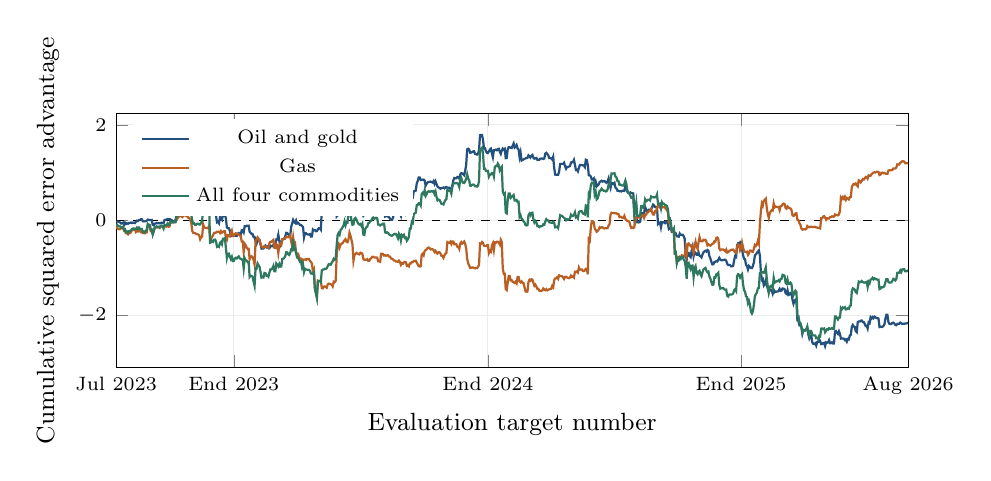
\begin{tikzpicture}
\begin{axis}[width=0.96\textwidth,height=4.8cm,xmin=0,xmax=801,
 xlabel={Evaluation target number},ylabel={Cumulative squared error advantage},
 xtick={0,119,376,632,801},xticklabels={Jul 2023,End 2023,End 2024,End 2025,Aug 2026},
 tick label style={font=\scriptsize},label style={font=\small},grid=major,grid style={gray!15},
 legend style={font=\scriptsize,at={(0.02,0.98)},anchor=north west,draw=none,fill=white}]
\addplot[black,dashed,thin,forget plot] coordinates {(0,0) (801,0)};
\addplot[reportblue,thick] coordinates {(0,-0.03294315) (1,-0.02688527) (2,-0.03249578) (3,-0.03691050) (4,-0.04845034) (5,-0.07019014) (6,-0.06534614) (7,-0.05251403) (8,-0.09770363) (9,-0.05213560) (10,-0.08009628) (11,-0.06420673) (12,-0.07628725) (13,-0.05827612) (14,-0.05777547) (15,-0.04921711) (16,-0.06139432) (17,-0.04983542) (18,-0.05408395) (19,-0.06054099) (20,-0.03240900) (21,-0.01034730) (22,-0.01839292) (23,0.00204004) (24,0.00370676) (25,0.01972062) (26,0.01950934) (27,-0.02310566) (28,-0.02567397) (29,-0.02418056) (30,-0.02280252) (31,-0.00808435) (32,0.01320653) (33,0.00778190) (34,0.00249048) (35,0.00183091) (36,0.00482727) (37,-0.09649803) (38,-0.10763602) (39,-0.07498952) (40,-0.07000614) (41,-0.05814364) (42,-0.06413583) (43,-0.06321574) (44,-0.06288332) (45,-0.05690262) (46,-0.05476930) (47,-0.05212065) (48,-0.06230196) (49,0.00636473) (50,0.00761174) (51,0.01257832) (52,0.02565895) (53,0.02045040) (54,0.02380793) (55,0.01221632) (56,0.00514729) (57,-0.01665122) (58,-0.02333552) (59,-0.01215457) (60,-0.01272822) (61,0.10103056) (62,0.06656869) (63,0.11118192) (64,0.11403790) (65,0.13074501) (66,0.14182319) (67,0.16017000) (68,0.15319507) (69,0.15578920) (70,0.13980300) (71,0.16218272) (72,0.16048312) (73,0.13436278) (74,0.12870042) (75,0.12825241) (76,0.13755871) (77,0.14098314) (78,0.13599364) (79,0.14920681) (80,0.13971572) (81,0.16282617) (82,0.19036675) (83,0.19002492) (84,0.18840888) (85,0.26580341) (86,0.26879419) (87,0.28288932) (88,0.47955681) (89,0.46021905) (90,0.45964107) (91,0.43116135) (92,0.43273111) (93,0.51485722) (94,0.51794929) (95,0.19945133) (96,0.20296418) (97,0.18707494) (98,0.13679702) (99,0.12793822) (100,0.13181736) (101,0.09577357) (102,-0.04347954) (103,-0.03029350) (104,-0.06395113) (105,0.06154571) (106,0.02189939) (107,0.00161983) (108,0.12188228) (109,0.09594923) (110,0.11049668) (111,0.03765727) (112,-0.15157543) (113,-0.17016389) (114,-0.16978853) (115,-0.22060795) (116,-0.33341019) (117,-0.32766997) (118,-0.32757037) (119,-0.32631097) (120,-0.32520957) (121,-0.32442495) (122,-0.32936982) (123,-0.28526032) (124,-0.26866529) (125,-0.28524652) (126,-0.29847254) (127,-0.21069261) (128,-0.21015525) (129,-0.25384206) (130,-0.12928940) (131,-0.13024552) (132,-0.11807945) (133,-0.11687685) (134,-0.11488829) (135,-0.24354312) (136,-0.26458900) (137,-0.28966891) (138,-0.29082677) (139,-0.35270149) (140,-0.35175151) (141,-0.44187549) (142,-0.49399548) (143,-0.41889835) (144,-0.41588246) (145,-0.41212138) (146,-0.50853277) (147,-0.59658792) (148,-0.59306740) (149,-0.59406777) (150,-0.54315221) (151,-0.53009459) (152,-0.56972404) (153,-0.55508504) (154,-0.58598436) (155,-0.58966765) (156,-0.53558923) (157,-0.54860940) (158,-0.54739554) (159,-0.51780160) (160,-0.49856298) (161,-0.49859910) (162,-0.40552207) (163,-0.40712201) (164,-0.30302727) (165,-0.43233158) (166,-0.53389439) (167,-0.49333217) (168,-0.40087396) (169,-0.39786188) (170,-0.39665105) (171,-0.34472013) (172,-0.26547880) (173,-0.26839931) (174,-0.29661281) (175,-0.31216373) (176,-0.33320264) (177,-0.14097957) (178,-0.07246070) (179,0.00539483) (180,-0.03683918) (181,-0.05731265) (182,-0.00706807) (183,-0.06867769) (184,-0.05556978) (185,-0.07314814) (186,-0.10199563) (187,-0.10202513) (188,-0.12046952) (189,-0.14176494) (190,-0.36008507) (191,-0.27298186) (192,-0.27374930) (193,-0.29118892) (194,-0.30059936) (195,-0.29945719) (196,-0.29181760) (197,-0.34344483) (198,-0.34065585) (199,-0.19551101) (200,-0.21340890) (201,-0.20979758) (202,-0.23151106) (203,-0.22884680) (204,-0.19337367) (205,-0.16864071) (206,-0.16766836) (207,-0.19731436) (208,0.21579652) (209,0.22123112) (210,0.20906500) (211,0.22180469) (212,0.23382280) (213,0.23637570) (214,0.23851130) (215,0.27001572) (216,0.27013739) (217,0.29636823) (218,0.34554222) (219,0.41941490) (220,0.38249484) (221,0.34509569) (222,0.35662765) (223,0.07776569) (224,0.10154500) (225,0.11030527) (226,0.11359056) (227,0.15243019) (228,0.13940608) (229,0.16759853) (230,0.16869173) (231,0.24705410) (232,0.16317719) (233,0.27534096) (234,0.27440220) (235,0.40004148) (236,0.32303176) (237,0.33898066) (238,0.28802029) (239,0.24916822) (240,0.50657617) (241,0.35058629) (242,0.33114634) (243,0.30043212) (244,0.23362806) (245,0.23116205) (246,0.22054530) (247,0.18496560) (248,0.17104769) (249,0.15198369) (250,0.09084732) (251,0.11372563) (252,0.28429492) (253,0.33238701) (254,0.31993149) (255,0.48802444) (256,0.49426934) (257,0.49310341) (258,0.50245145) (259,0.52057880) (260,0.51883405) (261,0.48323980) (262,0.49887313) (263,0.50727922) (264,0.49788664) (265,0.43274128) (266,0.43024327) (267,0.43535310) (268,0.27101362) (269,0.27065956) (270,0.27284090) (271,0.29794194) (272,0.07711873) (273,0.08746360) (274,0.08778830) (275,0.07435100) (276,0.06040956) (277,0.02972171) (278,0.00808426) (279,0.00864877) (280,0.05221271) (281,0.13862071) (282,0.14929003) (283,0.15477300) (284,0.14659313) (285,0.16243884) (286,0.14935279) (287,0.14271399) (288,0.08915787) (289,0.23529478) (290,0.22856902) (291,0.24252446) (292,0.20346530) (293,0.11722494) (294,0.13379200) (295,0.19255789) (296,0.22282371) (297,0.34887551) (298,0.34901238) (299,0.48955682) (300,0.47619102) (301,0.60294911) (302,0.61380034) (303,0.62044445) (304,0.76999196) (305,0.82200145) (306,0.89696075) (307,0.89595374) (308,0.84458380) (309,0.84547578) (310,0.84957484) (311,0.85141397) (312,0.83004751) (313,0.72490215) (314,0.76175101) (315,0.79235954) (316,0.80172001) (317,0.80340435) (318,0.80973842) (319,0.79781737) (320,0.78969657) (321,0.82007274) (322,0.76144613) (323,0.81335519) (324,0.75829430) (325,0.70737831) (326,0.68568984) (327,0.67614990) (328,0.65880354) (329,0.67333100) (330,0.67510169) (331,0.68501374) (332,0.66842957) (333,0.69047946) (334,0.69406479) (335,0.68204165) (336,0.67931689) (337,0.67937032) (338,0.66016378) (339,0.63907358) (340,0.72957805) (341,0.83394167) (342,0.88459622) (343,0.87712119) (344,0.87807309) (345,0.90551358) (346,0.89881020) (347,0.87332630) (348,0.95630641) (349,0.98582006) (350,0.98189830) (351,0.96534635) (352,0.94370474) (353,1.03901532) (354,1.15963316) (355,1.48602812) (356,1.49854470) (357,1.48574551) (358,1.41534288) (359,1.41730891) (360,1.42686767) (361,1.44222165) (362,1.44535685) (363,1.38617192) (364,1.38444918) (365,1.37495182) (366,1.39337788) (367,1.47182589) (368,1.78236469) (369,1.78891087) (370,1.78629889) (371,1.69328251) (372,1.50328235) (373,1.50613109) (374,1.44720422) (375,1.41109193) (376,1.41021642) (377,1.44033783) (378,1.48414371) (379,1.50121858) (380,1.40189346) (381,1.32064020) (382,1.46855053) (383,1.47056078) (384,1.47983650) (385,1.46598975) (386,1.49076156) (387,1.49670355) (388,1.43442042) (389,1.39119756) (390,1.46023297) (391,1.50090938) (392,1.47807417) (393,1.49555383) (394,1.30054549) (395,1.30446794) (396,1.48627693) (397,1.52978550) (398,1.52996486) (399,1.51711031) (400,1.51302889) (401,1.56367256) (402,1.60925499) (403,1.52242626) (404,1.54013597) (405,1.57525791) (406,1.50145148) (407,1.48451055) (408,1.32592350) (409,1.41866990) (410,1.25249415) (411,1.26466390) (412,1.27224302) (413,1.29087441) (414,1.29099439) (415,1.30634385) (416,1.30899966) (417,1.36008795) (418,1.33951464) (419,1.31295680) (420,1.35124571) (421,1.36779259) (422,1.31162753) (423,1.28957238) (424,1.29784563) (425,1.30516410) (426,1.26619711) (427,1.26956178) (428,1.26906607) (429,1.28917852) (430,1.29448431) (431,1.29287185) (432,1.28481922) (433,1.29300540) (434,1.39539806) (435,1.41245331) (436,1.39070110) (437,1.36230833) (438,1.30374216) (439,1.30245104) (440,1.29598133) (441,1.27155440) (442,1.32915289) (443,1.09636569) (444,0.95592695) (445,0.95351429) (446,0.95097424) (447,0.95086859) (448,1.01766509) (449,1.17801261) (450,1.18096042) (451,1.18109787) (452,1.18034304) (453,1.20504971) (454,1.13340912) (455,1.07930625) (456,1.11845572) (457,1.11513423) (458,1.12606101) (459,1.13507202) (460,1.21022924) (461,1.21809353) (462,1.21445150) (463,1.26309379) (464,1.16333157) (465,1.05277960) (466,1.06029526) (467,1.02411921) (468,1.09877436) (469,1.15727771) (470,1.15874058) (471,1.15373076) (472,1.15194248) (473,1.14365706) (474,1.11353715) (475,1.26732945) (476,1.25769493) (477,1.15830943) (478,0.94370058) (479,0.93991679) (480,0.91855981) (481,0.85222039) (482,0.85098635) (483,0.87444515) (484,0.74102393) (485,0.80436533) (486,0.70953958) (487,0.72938324) (488,0.75092317) (489,0.79884716) (490,0.81324884) (491,0.82756306) (492,0.80983223) (493,0.81592194) (494,0.81932969) (495,0.79680320) (496,0.78302844) (497,0.81503285) (498,0.87621448) (499,0.74845959) (500,0.67767643) (501,0.78368471) (502,0.77677440) (503,0.75877421) (504,0.77907509) (505,0.68176038) (506,0.66459253) (507,0.61770552) (508,0.61806351) (509,0.60656274) (510,0.60894160) (511,0.60265151) (512,0.61803127) (513,0.61909337) (514,0.61505169) (515,0.73984876) (516,0.70354342) (517,0.59508293) (518,0.56631642) (519,0.56455772) (520,0.58193677) (521,0.56911277) (522,0.56723168) (523,0.56110216) (524,0.20878181) (525,0.18070783) (526,0.27288920) (527,-0.04273661) (528,-0.04677742) (529,-0.04495055) (530,-0.03006900) (531,0.14387900) (532,0.14695167) (533,0.09193024) (534,0.15585201) (535,0.27487000) (536,0.22137192) (537,0.17863849) (538,0.19881884) (539,0.22010141) (540,0.21629602) (541,0.23295710) (542,0.27019843) (543,0.32664455) (544,0.31112589) (545,0.27500187) (546,0.27476736) (547,0.25857828) (548,-0.08040595) (549,-0.05924528) (550,-0.04953950) (551,-0.15062243) (552,-0.04342683) (553,-0.04476127) (554,-0.04385173) (555,-0.06153993) (556,-0.02777377) (557,-0.04416818) (558,-0.07975373) (559,-0.18763013) (560,-0.17279358) (561,-0.16199849) (562,-0.25016417) (563,-0.25062178) (564,-0.21118854) (565,-0.28378690) (566,-0.27923759) (567,-0.33882158) (568,-0.33862936) (569,-0.34672791) (570,-0.27992456) (571,-0.30744388) (572,-0.30967326) (573,-0.30638373) (574,-0.33714298) (575,-0.39039617) (576,-0.72669077) (577,-0.82980323) (578,-0.69369221) (579,-0.68717613) (580,-0.75100930) (581,-0.77474587) (582,-0.63805648) (583,-0.55837273) (584,-0.75490077) (585,-0.66804021) (586,-0.68295883) (587,-0.72670903) (588,-0.72725816) (589,-0.67433016) (590,-0.74451483) (591,-0.75865991) (592,-0.78124595) (593,-0.71956753) (594,-0.67513220) (595,-0.65243566) (596,-0.64012469) (597,-0.65734871) (598,-0.62595159) (599,-0.64071362) (600,-0.75395936) (601,-0.80369006) (602,-0.87442969) (603,-0.92724592) (604,-0.92398803) (605,-0.87612508) (606,-0.87516345) (607,-0.85964126) (608,-0.86614810) (609,-0.82603067) (610,-0.78997429) (611,-0.82735403) (612,-0.84006815) (613,-0.84033344) (614,-0.83535797) (615,-0.83191747) (616,-0.82876247) (617,-0.85143512) (618,-0.91655340) (619,-0.93982555) (620,-0.93727921) (621,-0.94527932) (622,-0.96893615) (623,-0.96800046) (624,-0.95735080) (625,-0.84133610) (626,-0.75475146) (627,-0.76953232) (628,-0.52626726) (629,-0.48376846) (630,-0.49206173) (631,-0.46580116) (632,-0.51267205) (633,-0.60678209) (634,-0.72965676) (635,-0.80853929) (636,-0.81795829) (637,-0.93822839) (638,-0.96157193) (639,-1.03333688) (640,-0.96019793) (641,-0.98330318) (642,-1.00374017) (643,-1.00449209) (644,-0.95974721) (645,-0.88053927) (646,-0.73938782) (647,-0.71412238) (648,-0.68878984) (649,-0.65752217) (650,-0.63372851) (651,-0.73479489) (652,-1.07256514) (653,-1.25432803) (654,-1.23659485) (655,-1.36762950) (656,-1.33464377) (657,-1.26235935) (658,-1.37291417) (659,-1.43021082) (660,-1.50640166) (661,-1.45644951) (662,-1.45890741) (663,-1.47570729) (664,-1.54066064) (665,-1.46148002) (666,-1.51048038) (667,-1.49560998) (668,-1.49873967) (669,-1.49746597) (670,-1.48074966) (671,-1.44104030) (672,-1.48097903) (673,-1.47520821) (674,-1.43271602) (675,-1.43985648) (676,-1.44716365) (677,-1.53050913) (678,-1.54536338) (679,-1.46676893) (680,-1.56759520) (681,-1.55574272) (682,-1.52733914) (683,-1.53676070) (684,-1.66802598) (685,-1.75042803) (686,-1.68834926) (687,-1.66977846) (688,-1.70029561) (689,-2.10177296) (690,-2.10568855) (691,-2.20180863) (692,-2.19241174) (693,-2.22913523) (694,-2.37921385) (695,-2.29981974) (696,-2.31460227) (697,-2.30930912) (698,-2.28412210) (699,-2.26625002) (700,-2.39189805) (701,-2.47579631) (702,-2.41844971) (703,-2.41902328) (704,-2.56285737) (705,-2.59112597) (706,-2.59398015) (707,-2.57937002) (708,-2.62919397) (709,-2.55356878) (710,-2.55374200) (711,-2.49936016) (712,-2.53286152) (713,-2.59911828) (714,-2.59831974) (715,-2.57667243) (716,-2.57121914) (717,-2.63960826) (718,-2.56092743) (719,-2.56857581) (720,-2.56496256) (721,-2.51539284) (722,-2.58072835) (723,-2.57868626) (724,-2.56023434) (725,-2.58506482) (726,-2.58433911) (727,-2.33360233) (728,-2.32394406) (729,-2.35870927) (730,-2.38514828) (731,-2.33130589) (732,-2.38684535) (733,-2.48368205) (734,-2.48031138) (735,-2.48099694) (736,-2.48476198) (737,-2.51453656) (738,-2.50059529) (739,-2.54579379) (740,-2.49165099) (741,-2.49979839) (742,-2.41621772) (743,-2.40456067) (744,-2.23684276) (745,-2.19725190) (746,-2.23108996) (747,-2.24069671) (748,-2.32518739) (749,-2.34758901) (750,-2.13750156) (751,-2.12443786) (752,-2.12500205) (753,-2.10740352) (754,-2.10290362) (755,-2.13355879) (756,-2.13472390) (757,-2.17141088) (758,-2.21897473) (759,-2.21364195) (760,-2.27045585) (761,-2.14417907) (762,-2.16046389) (763,-2.03559344) (764,-2.06235065) (765,-2.03084492) (766,-2.05438565) (767,-2.02387156) (768,-2.03829105) (769,-2.05086092) (770,-2.05637644) (771,-2.06243558) (772,-2.23998948) (773,-2.23182177) (774,-2.23595242) (775,-2.23878837) (776,-2.21780602) (777,-2.18543877) (778,-2.06213100) (779,-1.98368794) (780,-1.98278671) (781,-2.13174956) (782,-2.17273312) (783,-2.17968517) (784,-2.17390504) (785,-2.15323257) (786,-2.14865348) (787,-2.16488755) (788,-2.19544285) (789,-2.20220164) (790,-2.17365959) (791,-2.17175838) (792,-2.17348082) (793,-2.14729580) (794,-2.15965785) (795,-2.17617054) (796,-2.17337181) (797,-2.17253413) (798,-2.16562550) (799,-2.16593782) (800,-2.16075428) (801,-2.14422212)};\addlegendentry{Oil and gold}
\addplot[reportorange,thick] coordinates {(0,-0.11380282) (1,-0.17007630) (2,-0.18133874) (3,-0.19020888) (4,-0.18604088) (5,-0.17248088) (6,-0.16821138) (7,-0.16236890) (8,-0.22408175) (9,-0.23743274) (10,-0.27155119) (11,-0.27499863) (12,-0.29732761) (13,-0.27194221) (14,-0.26795995) (15,-0.25223946) (16,-0.20748543) (17,-0.20130428) (18,-0.19825175) (19,-0.19800808) (20,-0.24759436) (21,-0.22053139) (22,-0.23449535) (23,-0.20383354) (24,-0.22957296) (25,-0.25135526) (26,-0.25431537) (27,-0.26966404) (28,-0.26846514) (29,-0.27511758) (30,-0.25724287) (31,-0.25500352) (32,-0.10366464) (33,-0.11162234) (34,-0.11143537) (35,-0.23450214) (36,-0.23404531) (37,-0.28414915) (38,-0.22676730) (39,-0.16398012) (40,-0.15407751) (41,-0.15071396) (42,-0.15333516) (43,-0.15215719) (44,-0.16163094) (45,-0.13386332) (46,-0.13139147) (47,-0.13669010) (48,-0.16256557) (49,-0.12493458) (50,-0.12855693) (51,-0.13527174) (52,-0.11629619) (53,-0.13718590) (54,-0.13091851) (55,-0.04711362) (56,-0.04809050) (57,-0.04310114) (58,-0.03972567) (59,-0.03926541) (60,-0.03917105) (61,-0.00484959) (62,0.03890129) (63,0.06779933) (64,0.07939045) (65,0.08140027) (66,0.07956520) (67,0.06509691) (68,0.08767476) (69,0.10528038) (70,0.10873623) (71,0.08344549) (72,0.08372760) (73,0.04948819) (74,0.04632953) (75,-0.00619507) (76,-0.05668694) (77,-0.22449329) (78,-0.26534176) (79,-0.26777217) (80,-0.27420490) (81,-0.28905149) (82,-0.29662558) (83,-0.29878747) (84,-0.31780487) (85,-0.40104706) (86,-0.36040635) (87,-0.33957070) (88,-0.08698174) (89,-0.14938289) (90,-0.15938282) (91,-0.16498965) (92,-0.16364871) (93,-0.17023626) (94,-0.11827511) (95,-0.40084758) (96,-0.39524559) (97,-0.34397266) (98,-0.32046076) (99,-0.26558293) (100,-0.26273305) (101,-0.26081935) (102,-0.24262818) (103,-0.24273978) (104,-0.24129235) (105,-0.26901390) (106,-0.23002176) (107,-0.26209670) (108,-0.24411772) (109,-0.23050167) (110,-0.22989133) (111,-0.36281145) (112,-0.40901325) (113,-0.31153055) (114,-0.31546980) (115,-0.33545046) (116,-0.27296147) (117,-0.22153533) (118,-0.33320855) (119,-0.32980239) (120,-0.29011368) (121,-0.27303879) (122,-0.28616178) (123,-0.29652355) (124,-0.29438648) (125,-0.32429315) (126,-0.32585023) (127,-0.44788050) (128,-0.44795004) (129,-0.66666108) (130,-0.49593275) (131,-0.52382376) (132,-0.57023890) (133,-0.60320468) (134,-0.60058920) (135,-0.81607703) (136,-0.76233620) (137,-0.75630525) (138,-0.77949784) (139,-0.83227859) (140,-0.93691572) (141,-0.43735142) (142,-0.40300106) (143,-0.36026941) (144,-0.38781128) (145,-0.44313254) (146,-0.48440794) (147,-0.55652546) (148,-0.57207433) (149,-0.57188836) (150,-0.54624108) (151,-0.55363668) (152,-0.56191918) (153,-0.56014373) (154,-0.57935614) (155,-0.48264337) (156,-0.45055404) (157,-0.45299567) (158,-0.43056567) (159,-0.41320030) (160,-0.57842727) (161,-0.58308576) (162,-0.49753087) (163,-0.53312815) (164,-0.68593063) (165,-0.52451789) (166,-0.49142951) (167,-0.51658353) (168,-0.40319054) (169,-0.39645041) (170,-0.37797827) (171,-0.38455784) (172,-0.35040715) (173,-0.35272344) (174,-0.35638564) (175,-0.35664115) (176,-0.32305921) (177,-0.44422038) (178,-0.53697924) (179,-0.36441566) (180,-0.52714710) (181,-0.49448732) (182,-0.68986246) (183,-0.69630138) (184,-0.70191934) (185,-0.76923602) (186,-0.81912881) (187,-0.81146597) (188,-0.90424843) (189,-0.82620190) (190,-0.82739022) (191,-0.82225035) (192,-0.83437788) (193,-0.81476303) (194,-0.81503848) (195,-0.81419170) (196,-0.85507282) (197,-0.87304890) (198,-0.90748500) (199,-1.07387173) (200,-1.03258479) (201,-1.43596642) (202,-1.49878039) (203,-1.61082471) (204,-1.26642725) (205,-1.27742500) (206,-1.27648580) (207,-1.26815390) (208,-1.42427145) (209,-1.42980538) (210,-1.39408304) (211,-1.38752641) (212,-1.40225986) (213,-1.41697892) (214,-1.34436936) (215,-1.32944390) (216,-1.33405670) (217,-1.34643987) (218,-1.34757438) (219,-1.38644545) (220,-1.29038826) (221,-1.30223487) (222,-1.27353140) (223,-0.77163379) (224,-0.53986152) (225,-0.49919411) (226,-0.57517509) (227,-0.51153438) (228,-0.49020066) (229,-0.48421386) (230,-0.44976038) (231,-0.42136234) (232,-0.39887598) (233,-0.45197545) (234,-0.46096731) (235,-0.40099855) (236,-0.26089562) (237,-0.32305194) (238,-0.41252254) (239,-0.50580689) (240,-0.84889738) (241,-0.73182736) (242,-0.70896680) (243,-0.68584938) (244,-0.70076661) (245,-0.71336537) (246,-0.71809801) (247,-0.68250226) (248,-0.68838883) (249,-0.70428049) (250,-0.81052881) (251,-0.83419265) (252,-0.83012441) (253,-0.83075625) (254,-0.81833821) (255,-0.85752485) (256,-0.85379977) (257,-0.81217114) (258,-0.79759621) (259,-0.76819897) (260,-0.76880533) (261,-0.77943014) (262,-0.78226498) (263,-0.78194402) (264,-0.78492389) (265,-0.86078669) (266,-0.86151657) (267,-0.87136467) (268,-0.70299457) (269,-0.70297641) (270,-0.71095476) (271,-0.74132080) (272,-0.73594461) (273,-0.74542326) (274,-0.73736366) (275,-0.73679581) (276,-0.76367941) (277,-0.76430914) (278,-0.80358455) (279,-0.80636573) (280,-0.81999754) (281,-0.84701066) (282,-0.84864965) (283,-0.86649803) (284,-0.86828228) (285,-0.87332825) (286,-0.84803972) (287,-0.87383240) (288,-0.93731510) (289,-0.90416165) (290,-0.91457798) (291,-0.88556693) (292,-0.87570452) (293,-0.88205965) (294,-0.95599030) (295,-0.94591401) (296,-0.96815121) (297,-0.90904961) (298,-0.90825104) (299,-0.87712774) (300,-0.87948936) (301,-0.85688543) (302,-0.85527743) (303,-0.84885733) (304,-0.88902431) (305,-0.92683305) (306,-0.96499310) (307,-0.97214566) (308,-0.96608334) (309,-0.72654052) (310,-0.70315465) (311,-0.73591425) (312,-0.64526670) (313,-0.62723721) (314,-0.61187013) (315,-0.58226493) (316,-0.57315932) (317,-0.58402468) (318,-0.61334579) (319,-0.61186646) (320,-0.60812392) (321,-0.62322966) (322,-0.66503582) (323,-0.64283059) (324,-0.68630629) (325,-0.69830465) (326,-0.67290542) (327,-0.67293909) (328,-0.69706752) (329,-0.74695732) (330,-0.74820877) (331,-0.78885672) (332,-0.73806478) (333,-0.70026479) (334,-0.68596999) (335,-0.45948591) (336,-0.47176842) (337,-0.47376995) (338,-0.45099842) (339,-0.49902723) (340,-0.44818214) (341,-0.44643177) (342,-0.50433631) (343,-0.49755391) (344,-0.50374833) (345,-0.55456985) (346,-0.56071491) (347,-0.60395717) (348,-0.49033020) (349,-0.46050965) (350,-0.48990568) (351,-0.47066285) (352,-0.44872686) (353,-0.49464377) (354,-0.59226207) (355,-0.80660477) (356,-0.90465398) (357,-0.94712829) (358,-1.00054726) (359,-0.99862233) (360,-0.98936918) (361,-0.99434154) (362,-1.00287020) (363,-1.01007261) (364,-1.00146443) (365,-1.00548455) (366,-0.97709121) (367,-0.93825819) (368,-0.48789131) (369,-0.49334003) (370,-0.45798523) (371,-0.47782569) (372,-0.53367843) (373,-0.54199608) (374,-0.54244347) (375,-0.52498988) (376,-0.52136097) (377,-0.68723102) (378,-0.64112339) (379,-0.66120915) (380,-0.53344383) (381,-0.48551858) (382,-0.62247411) (383,-0.46499782) (384,-0.47088697) (385,-0.45149520) (386,-0.45410910) (387,-0.47262719) (388,-0.51085931) (389,-0.41208679) (390,-0.45850605) (391,-1.00639355) (392,-1.12243910) (393,-1.12275686) (394,-1.44693532) (395,-1.46561131) (396,-1.31200984) (397,-1.17094051) (398,-1.17139038) (399,-1.26117786) (400,-1.25672688) (401,-1.29221599) (402,-1.30128668) (403,-1.31565302) (404,-1.29033696) (405,-1.32362838) (406,-1.19155600) (407,-1.19180388) (408,-1.28550938) (409,-1.30363331) (410,-1.28174061) (411,-1.31457300) (412,-1.31975188) (413,-1.40252573) (414,-1.49203796) (415,-1.50199000) (416,-1.49542258) (417,-1.29273995) (418,-1.25003714) (419,-1.26983803) (420,-1.23913481) (421,-1.24570142) (422,-1.31413247) (423,-1.37574239) (424,-1.35057413) (425,-1.39312980) (426,-1.44110216) (427,-1.43926072) (428,-1.47908172) (429,-1.48041342) (430,-1.47876171) (431,-1.47572095) (432,-1.43380977) (433,-1.45400520) (434,-1.46915719) (435,-1.44538986) (436,-1.46993296) (437,-1.45989486) (438,-1.44923231) (439,-1.44407241) (440,-1.43875611) (441,-1.37798797) (442,-1.40677733) (443,-1.25666651) (444,-1.22103328) (445,-1.21636798) (446,-1.19750331) (447,-1.22914300) (448,-1.15802927) (449,-1.16741345) (450,-1.17400365) (451,-1.17483262) (452,-1.19818183) (453,-1.23309690) (454,-1.19046920) (455,-1.18593938) (456,-1.20097302) (457,-1.20970145) (458,-1.21590584) (459,-1.20403400) (460,-1.16190286) (461,-1.18991766) (462,-1.17833619) (463,-1.20073273) (464,-1.08220071) (465,-1.08437751) (466,-1.07374750) (467,-1.09648344) (468,-0.99384091) (469,-1.03791847) (470,-1.03339935) (471,-1.03308600) (472,-1.06666962) (473,-1.06725155) (474,-1.05451944) (475,-1.01559208) (476,-1.01547421) (477,-1.13618367) (478,-0.39806500) (479,-0.42649587) (480,-0.16916811) (481,-0.02185453) (482,-0.02372524) (483,-0.04377968) (484,-0.17467826) (485,-0.20399449) (486,-0.24245160) (487,-0.22568145) (488,-0.19763229) (489,-0.14752409) (490,-0.16190879) (491,-0.14727927) (492,-0.15102356) (493,-0.16930814) (494,-0.17244214) (495,-0.16855611) (496,-0.16823589) (497,-0.16478296) (498,-0.11328221) (499,-0.08232254) (500,0.11682507) (501,0.15652420) (502,0.15031400) (503,0.15151226) (504,0.14506921) (505,0.14676114) (506,0.14307405) (507,0.13082548) (508,0.13074870) (509,0.06658876) (510,0.07028341) (511,0.06635788) (512,0.04425827) (513,0.04519741) (514,0.08877275) (515,0.02598058) (516,0.00059797) (517,-0.01742853) (518,-0.01965517) (519,-0.03445375) (520,-0.10968584) (521,-0.16228142) (522,-0.15214559) (523,-0.16133135) (524,-0.15096597) (525,-0.02126999) (526,0.06137822) (527,0.06099065) (528,0.06100546) (529,0.05726317) (530,0.06658673) (531,0.09758994) (532,0.09832596) (533,0.10915219) (534,0.05099388) (535,0.10915518) (536,0.11592204) (537,0.16383718) (538,0.16462344) (539,0.18785212) (540,0.19856308) (541,0.23158719) (542,0.16616940) (543,0.11891241) (544,0.11915013) (545,0.18785524) (546,0.18452539) (547,0.24608789) (548,0.31522441) (549,0.29460823) (550,0.26395088) (551,0.24206107) (552,0.29050871) (553,0.27106282) (554,0.27327767) (555,0.26975141) (556,0.22870304) (557,0.22319702) (558,0.16372328) (559,-0.03516163) (560,-0.03101215) (561,-0.13875259) (562,-0.23468904) (563,-0.23609878) (564,-0.21596237) (565,-0.69772980) (566,-0.68610239) (567,-0.85873738) (568,-0.77176316) (569,-0.78140249) (570,-0.78422358) (571,-0.79160249) (572,-0.73662599) (573,-0.74182929) (574,-0.76596881) (575,-0.75472503) (576,-0.59085040) (577,-0.72198136) (578,-0.49954327) (579,-0.48926754) (580,-0.51789207) (581,-0.54444758) (582,-0.53133704) (583,-0.61669197) (584,-0.68591001) (585,-0.53993256) (586,-0.45385728) (587,-0.55769183) (588,-0.60091248) (589,-0.46506808) (590,-0.35620845) (591,-0.43160859) (592,-0.44133078) (593,-0.44054701) (594,-0.41114644) (595,-0.41770058) (596,-0.41193236) (597,-0.45481760) (598,-0.52710520) (599,-0.50539948) (600,-0.52169216) (601,-0.53466564) (602,-0.51452723) (603,-0.49349560) (604,-0.49091354) (605,-0.44170464) (606,-0.44729692) (607,-0.37031872) (608,-0.36174567) (609,-0.39323076) (610,-0.59187920) (611,-0.62761875) (612,-0.61234267) (613,-0.61298694) (614,-0.61245405) (615,-0.63120597) (616,-0.65104182) (617,-0.61530796) (618,-0.67898368) (619,-0.67107344) (620,-0.64581733) (621,-0.63597317) (622,-0.62072784) (623,-0.61919128) (624,-0.61658832) (625,-0.64454979) (626,-0.67906469) (627,-0.68985212) (628,-0.56115372) (629,-0.50941633) (630,-0.51913841) (631,-0.63108873) (632,-0.58568134) (633,-0.47225001) (634,-0.57057024) (635,-0.64989802) (636,-0.66121740) (637,-0.66304494) (638,-0.65942487) (639,-0.72789698) (640,-0.69842290) (641,-0.63798932) (642,-0.63722838) (643,-0.65693165) (644,-0.66310135) (645,-0.59475854) (646,-0.51796204) (647,-0.54031204) (648,-0.51230989) (649,-0.43325401) (650,-0.49437890) (651,-0.09034906) (652,0.17631749) (653,0.35207702) (654,0.31008468) (655,0.41000398) (656,0.42599371) (657,0.45089222) (658,0.25553149) (659,0.13377192) (660,0.04733709) (661,0.14057273) (662,0.18465624) (663,0.21017531) (664,0.20189968) (665,0.35064514) (666,0.26938238) (667,0.28778476) (668,0.27768932) (669,0.27933581) (670,0.27713428) (671,0.20966064) (672,0.29361872) (673,0.29886788) (674,0.33240050) (675,0.34743392) (676,0.34036770) (677,0.25761052) (678,0.24231028) (679,0.28841015) (680,0.26880301) (681,0.24993405) (682,0.24592001) (683,0.21357414) (684,0.10350631) (685,0.08818143) (686,0.10444562) (687,0.14299868) (688,0.14433011) (689,0.00755710) (690,-0.00118052) (691,-0.06365624) (692,-0.09212875) (693,-0.17482197) (694,-0.19833507) (695,-0.19116284) (696,-0.19166941) (697,-0.19376192) (698,-0.18235746) (699,-0.12321590) (700,-0.14234393) (701,-0.14936608) (702,-0.13765705) (703,-0.13772665) (704,-0.14363767) (705,-0.14331247) (706,-0.14391671) (707,-0.14033242) (708,-0.15444646) (709,-0.15352511) (710,-0.16044066) (711,-0.16307789) (712,-0.17261172) (713,0.04109240) (714,0.04130676) (715,0.07515819) (716,0.08502123) (717,0.05191469) (718,0.01134082) (719,0.04237720) (720,0.03314076) (721,0.03286259) (722,0.06337107) (723,0.06513007) (724,0.08216346) (725,0.07340431) (726,0.07452763) (727,0.12012316) (728,0.10670474) (729,0.11198565) (730,0.10207497) (731,0.11844766) (732,0.19198760) (733,0.47648205) (734,0.44735298) (735,0.48713416) (736,0.45086254) (737,0.49029409) (738,0.42768422) (739,0.46663621) (740,0.45558313) (741,0.43601228) (742,0.48291913) (743,0.48564491) (744,0.69281103) (745,0.73728630) (746,0.76009736) (747,0.74953711) (748,0.76893310) (749,0.73353039) (750,0.71008550) (751,0.83690924) (752,0.82415734) (753,0.79251744) (754,0.82035370) (755,0.86093122) (756,0.85275994) (757,0.87324469) (758,0.90487392) (759,0.90738858) (760,0.87169140) (761,0.94151350) (762,0.92966120) (763,0.93214930) (764,0.96810466) (765,0.98142594) (766,1.00227802) (767,1.00334982) (768,1.00080312) (769,1.01600600) (770,1.01554892) (771,1.01254375) (772,0.94671433) (773,0.95551704) (774,0.99479397) (775,0.99789719) (776,0.98437320) (777,0.99095341) (778,0.97612601) (779,0.97217219) (780,0.97319164) (781,1.03863193) (782,1.04677565) (783,1.04919235) (784,1.04635082) (785,1.05155923) (786,1.08544496) (787,1.08574723) (788,1.08423928) (789,1.10218543) (790,1.17066000) (791,1.16749915) (792,1.16799659) (793,1.20777235) (794,1.21288094) (795,1.23818681) (796,1.23500002) (797,1.22958615) (798,1.19547369) (799,1.19465932) (800,1.19780813) (801,1.18843573)};\addlegendentry{Gas}
\addplot[reportgreen,thick] coordinates {(0,-0.07797002) (1,-0.09991178) (2,-0.11827566) (3,-0.12701074) (4,-0.13264167) (5,-0.15446068) (6,-0.15007881) (7,-0.13729716) (8,-0.20260605) (9,-0.19160892) (10,-0.25184132) (11,-0.23564000) (12,-0.26028157) (13,-0.22801894) (14,-0.23011961) (15,-0.21772040) (16,-0.18362130) (17,-0.17698326) (18,-0.17407273) (19,-0.18241869) (20,-0.18819905) (21,-0.15439889) (22,-0.18100916) (23,-0.15344954) (24,-0.18127064) (25,-0.18353182) (26,-0.18566476) (27,-0.23959045) (28,-0.23670164) (29,-0.25679623) (30,-0.21867164) (31,-0.20351091) (32,-0.07756203) (33,-0.09629953) (34,-0.09895770) (35,-0.19659966) (36,-0.19475527) (37,-0.30199480) (38,-0.23454918) (39,-0.15253153) (40,-0.13985601) (41,-0.12872444) (42,-0.13579834) (43,-0.13708515) (44,-0.15494884) (45,-0.11367294) (46,-0.11191754) (47,-0.12333920) (48,-0.17286496) (49,-0.10117348) (50,-0.10504746) (51,-0.10699019) (52,-0.06712778) (53,-0.09580336) (54,-0.08902784) (55,-0.02242310) (56,-0.02802395) (57,-0.04355098) (58,-0.04990714) (59,-0.04247960) (60,-0.04245538) (61,0.09163553) (62,0.08455459) (63,0.13399975) (64,0.14756507) (65,0.16815952) (66,0.17200278) (67,0.18821206) (68,0.21798692) (69,0.24040644) (70,0.24750243) (71,0.25064913) (72,0.25116477) (73,0.18809856) (74,0.18693514) (75,0.14891040) (76,0.10804506) (77,-0.00900595) (78,-0.07230705) (79,-0.06661884) (80,-0.09959116) (81,-0.09364144) (82,-0.07385919) (83,-0.07536503) (84,-0.09255076) (85,-0.09222756) (86,-0.04862677) (87,-0.02664818) (88,0.33321552) (89,0.28789773) (90,0.26686138) (91,0.25193039) (92,0.24820794) (93,0.34437107) (94,0.33435062) (95,-0.47234149) (96,-0.46373116) (97,-0.43326531) (98,-0.45180501) (99,-0.41053011) (100,-0.40674546) (101,-0.44296820) (102,-0.55801035) (103,-0.54655610) (104,-0.55996862) (105,-0.47334806) (106,-0.45563204) (107,-0.50274800) (108,-0.38980552) (109,-0.39084446) (110,-0.37656189) (111,-0.58278910) (112,-0.79377024) (113,-0.70196801) (114,-0.69976521) (115,-0.76562479) (116,-0.81519905) (117,-0.76789677) (118,-0.85689082) (119,-0.85327845) (120,-0.80503162) (121,-0.78816957) (122,-0.80204126) (123,-0.77779654) (124,-0.76057475) (125,-0.80076036) (126,-0.80827852) (127,-0.82501442) (128,-0.82609843) (129,-1.01079077) (130,-0.79847258) (131,-0.83879747) (132,-0.84664628) (133,-0.87918660) (134,-0.87766358) (135,-1.19006236) (136,-1.16365347) (137,-1.17158488) (138,-1.18238369) (139,-1.29045354) (140,-1.37715898) (141,-1.01455881) (142,-1.01745779) (143,-0.90728776) (144,-0.94404679) (145,-0.97510579) (146,-1.08284212) (147,-1.20486651) (148,-1.19381745) (149,-1.20123334) (150,-1.10766496) (151,-1.11265466) (152,-1.16317199) (153,-1.16137344) (154,-1.18328340) (155,-1.10008456) (156,-1.03240067) (157,-1.03513676) (158,-1.01023311) (159,-0.96092784) (160,-1.06886307) (161,-1.07150147) (162,-0.90756805) (163,-0.93465355) (164,-0.96883262) (165,-0.91890560) (166,-0.97457564) (167,-0.97151533) (168,-0.81497456) (169,-0.80774322) (170,-0.79064499) (171,-0.75730770) (172,-0.67399649) (173,-0.67478385) (174,-0.71460896) (175,-0.72926451) (176,-0.68597755) (177,-0.61605371) (178,-0.62564808) (179,-0.40088996) (180,-0.60876647) (181,-0.59311158) (182,-0.70090286) (183,-0.78268789) (184,-0.78612233) (185,-0.83114749) (186,-0.87574820) (187,-0.86820971) (188,-0.98301329) (189,-0.92672492) (190,-1.08815028) (191,-1.01915436) (192,-1.03548323) (193,-1.03700602) (194,-1.04230728) (195,-1.04138764) (196,-1.06074963) (197,-1.11983269) (198,-1.12070410) (199,-1.12587668) (200,-1.09767664) (201,-1.43614837) (202,-1.53707395) (203,-1.62920458) (204,-1.29726770) (205,-1.27702294) (206,-1.27618533) (207,-1.29527837) (208,-1.05151733) (209,-1.03792664) (210,-1.03262013) (211,-1.01766874) (212,-1.01908718) (213,-1.00871114) (214,-0.96451568) (215,-0.92180152) (216,-0.92704294) (217,-0.93411912) (218,-0.89379622) (219,-0.86115974) (220,-0.80979421) (221,-0.83090662) (222,-0.80418577) (223,-0.53776180) (224,-0.30621846) (225,-0.26766382) (226,-0.30352048) (227,-0.20654494) (228,-0.18326217) (229,-0.14730802) (230,-0.11109782) (231,-0.02711436) (232,-0.10628924) (233,-0.03767081) (234,-0.04831450) (235,0.13817578) (236,0.15022053) (237,0.14680624) (238,-0.00625967) (239,-0.09606843) (240,-0.08891085) (241,0.02385588) (242,0.04625983) (243,0.01440065) (244,-0.03913753) (245,-0.07360897) (246,-0.09216378) (247,-0.07998759) (248,-0.11658947) (249,-0.07727048) (250,-0.30031404) (251,-0.30990710) (252,-0.18214799) (253,-0.14936273) (254,-0.13466208) (255,-0.06382266) (256,-0.05562620) (257,-0.02275636) (258,-0.00965010) (259,0.03887744) (260,0.05575746) (261,0.02849056) (262,0.04229407) (263,0.05099601) (264,0.04320022) (265,-0.09039054) (266,-0.09339213) (267,-0.10973321) (268,-0.09276025) (269,-0.09257511) (270,-0.07188794) (271,-0.07342546) (272,-0.25565466) (273,-0.26320646) (274,-0.25407471) (275,-0.26694421) (276,-0.29627669) (277,-0.30978404) (278,-0.32408372) (279,-0.32465080) (280,-0.31015515) (281,-0.29446109) (282,-0.28640423) (283,-0.28987695) (284,-0.33015507) (285,-0.37853841) (286,-0.28075514) (287,-0.31438194) (288,-0.42634153) (289,-0.31213072) (290,-0.33440367) (291,-0.30839490) (292,-0.37253842) (293,-0.36370909) (294,-0.43112141) (295,-0.40187330) (296,-0.35419275) (297,-0.17392937) (298,-0.17524404) (299,-0.03420092) (300,-0.05596150) (301,0.12725192) (302,0.14534167) (303,0.15619951) (304,0.31276633) (305,0.31750274) (306,0.35488698) (307,0.35111744) (308,0.31177963) (309,0.55001045) (310,0.57387957) (311,0.54908684) (312,0.62706570) (313,0.51028273) (314,0.54486509) (315,0.59469531) (316,0.60797199) (317,0.59442748) (318,0.60195708) (319,0.61054447) (320,0.59878274) (321,0.60992582) (322,0.55049716) (323,0.60119817) (324,0.48970043) (325,0.41535697) (326,0.43147124) (327,0.42609359) (328,0.38528707) (329,0.34195111) (330,0.34066779) (331,0.32986605) (332,0.38006779) (333,0.42123993) (334,0.44047301) (335,0.64143005) (336,0.61800938) (337,0.61456945) (338,0.62176484) (339,0.55776832) (340,0.69590072) (341,0.76692870) (342,0.77772351) (343,0.77460818) (344,0.78009465) (345,0.77246153) (346,0.75266152) (347,0.69692157) (348,0.86096561) (349,0.89030982) (350,0.81067458) (351,0.78341228) (352,0.77882643) (353,0.81700680) (354,0.86900116) (355,0.96296894) (356,0.87635994) (357,0.83812114) (358,0.72427352) (359,0.72404533) (360,0.74002399) (361,0.74860424) (362,0.74204119) (363,0.71172057) (364,0.71360203) (365,0.70389343) (366,0.72213940) (367,0.82313833) (368,1.49227504) (369,1.49425234) (370,1.51726829) (371,1.40706586) (372,1.07974311) (373,1.08167318) (374,1.03286228) (375,1.02858922) (376,1.03213000) (377,0.91495856) (378,0.95772489) (379,0.95811581) (380,0.98965065) (381,0.98963550) (382,0.91628127) (383,1.12030879) (384,1.13750087) (385,1.13120036) (386,1.18712368) (387,1.15022015) (388,1.04748185) (389,1.09052144) (390,1.11774341) (391,0.60439445) (392,0.54703652) (393,0.56449855) (394,0.16062288) (395,0.14417447) (396,0.42071967) (397,0.56166623) (398,0.56134375) (399,0.46613274) (400,0.48754602) (401,0.50605708) (402,0.52789666) (403,0.41065325) (404,0.41059016) (405,0.42281164) (406,0.38144763) (407,0.38744221) (408,0.06856917) (409,0.10260767) (410,0.03088698) (411,0.01685806) (412,-0.02630881) (413,-0.04484294) (414,-0.10054522) (415,-0.11206663) (416,-0.10390656) (417,0.10421715) (418,0.13654000) (419,0.10165259) (420,0.15357056) (421,0.15792666) (422,0.01815890) (423,-0.04998709) (424,-0.01681679) (425,-0.04421315) (426,-0.12449116) (427,-0.12260525) (428,-0.14556836) (429,-0.13017869) (430,-0.12591037) (431,-0.12242875) (432,-0.08830263) (433,-0.09388319) (434,-0.02866509) (435,0.02079871) (436,-0.00329684) (437,-0.00598977) (438,-0.04459596) (439,-0.04807521) (440,-0.05264314) (441,-0.05535252) (442,-0.03167036) (443,-0.05790343) (444,-0.15066962) (445,-0.14942695) (446,-0.13620511) (447,-0.16504659) (448,-0.04165657) (449,0.10280259) (450,0.09234863) (451,0.09016670) (452,0.06721973) (453,0.04791088) (454,0.03211862) (455,-0.00012707) (456,0.02178752) (457,0.01120835) (458,0.01729999) (459,0.03691490) (460,0.11453421) (461,0.09010975) (462,0.08920031) (463,0.10970657) (464,0.16458115) (465,0.06076385) (466,0.07738827) (467,0.04137345) (468,0.17156463) (469,0.18602633) (470,0.18921744) (471,0.18585552) (472,0.13857338) (473,0.13448677) (474,0.12143567) (475,0.30827596) (476,0.29809574) (477,0.06168336) (478,0.54577807) (479,0.50163440) (480,0.72645059) (481,0.78538189) (482,0.77932018) (483,0.79361536) (484,0.53419788) (485,0.58608547) (486,0.43787984) (487,0.45896685) (488,0.53094683) (489,0.61666988) (490,0.62016747) (491,0.66071176) (492,0.63510419) (493,0.61780039) (494,0.62004491) (495,0.60259996) (496,0.60509379) (497,0.64466889) (498,0.73836576) (499,0.72448426) (500,0.84521006) (501,0.97898610) (502,0.97842161) (503,0.97647417) (504,0.98479342) (505,0.91328816) (506,0.89815061) (507,0.82141701) (508,0.82176838) (509,0.74284699) (510,0.74643338) (511,0.73383178) (512,0.72633096) (513,0.72557075) (514,0.76602671) (515,0.83159380) (516,0.75901950) (517,0.62014430) (518,0.57616123) (519,0.56552626) (520,0.51631074) (521,0.47010997) (522,0.47758366) (523,0.46301545) (524,0.09589722) (525,0.22165356) (526,0.36723050) (527,0.09479546) (528,0.09264861) (529,0.09110451) (530,0.11513379) (531,0.29599037) (532,0.29783929) (533,0.26375190) (534,0.29544650) (535,0.43640821) (536,0.39557012) (537,0.41038301) (538,0.43015565) (539,0.43083854) (540,0.41353441) (541,0.49654053) (542,0.48015973) (543,0.48663684) (544,0.47740158) (545,0.48202852) (546,0.48197681) (547,0.53881326) (548,0.34914243) (549,0.34135242) (550,0.34928369) (551,0.25092000) (552,0.37888215) (553,0.34536511) (554,0.34479901) (555,0.31724938) (556,0.31394189) (557,0.29854996) (558,0.23217278) (559,0.02276546) (560,0.03477777) (561,-0.06602063) (562,-0.21842760) (563,-0.21858465) (564,-0.17958597) (565,-0.68757012) (566,-0.67361413) (567,-0.90327633) (568,-0.81847687) (569,-0.83935294) (570,-0.78178256) (571,-0.81326779) (572,-0.77105431) (573,-0.77206868) (574,-0.82486645) (575,-0.85544270) (576,-0.97716871) (577,-1.22781271) (578,-0.90318115) (579,-0.89337761) (580,-0.97361662) (581,-1.02789932) (582,-0.95354314) (583,-0.95132172) (584,-1.19102068) (585,-1.01312952) (586,-0.96616504) (587,-1.10663787) (588,-1.13340644) (589,-1.08055026) (590,-1.06054881) (591,-1.13848458) (592,-1.17462016) (593,-1.09371043) (594,-1.03218370) (595,-1.01299423) (596,-1.00040991) (597,-1.06055749) (598,-1.09135435) (599,-1.07823348) (600,-1.18114715) (601,-1.22730023) (602,-1.29903237) (603,-1.35518177) (604,-1.35029156) (605,-1.19907895) (606,-1.20384812) (607,-1.13361901) (608,-1.12763268) (609,-1.10384959) (610,-1.35984837) (611,-1.43707695) (612,-1.42743868) (613,-1.42786386) (614,-1.42343696) (615,-1.44622729) (616,-1.45663204) (617,-1.45573781) (618,-1.58395316) (619,-1.60113483) (620,-1.56085815) (621,-1.55614440) (622,-1.55711859) (623,-1.55550691) (624,-1.53951744) (625,-1.46976318) (626,-1.44527096) (627,-1.48301340) (628,-1.17144916) (629,-1.13148503) (630,-1.14470899) (631,-1.19893367) (632,-1.15614367) (633,-1.13010634) (634,-1.34122483) (635,-1.46946840) (636,-1.49630098) (637,-1.59552917) (638,-1.61185888) (639,-1.73821789) (640,-1.69169073) (641,-1.76972858) (642,-1.92141851) (643,-1.95760342) (644,-1.90942275) (645,-1.77356559) (646,-1.59138765) (647,-1.54988441) (648,-1.51995634) (649,-1.42926782) (650,-1.42255566) (651,-1.11617428) (652,-1.12426233) (653,-1.08434937) (654,-1.09290146) (655,-1.10197824) (656,-1.06163759) (657,-0.99197378) (658,-1.22203818) (659,-1.38464815) (660,-1.51837485) (661,-1.41121751) (662,-1.37807451) (663,-1.36963200) (664,-1.43052997) (665,-1.20825357) (666,-1.30995240) (667,-1.29411193) (668,-1.28103118) (669,-1.27911278) (670,-1.25838578) (671,-1.28368665) (672,-1.23585670) (673,-1.22769986) (674,-1.14491336) (675,-1.15199629) (676,-1.16733510) (677,-1.31258748) (678,-1.33293751) (679,-1.24471457) (680,-1.33683179) (681,-1.33419280) (682,-1.30994195) (683,-1.34068122) (684,-1.51728070) (685,-1.57140613) (686,-1.52436555) (687,-1.47984534) (688,-1.50679487) (689,-2.00570170) (690,-2.00797934) (691,-2.14542141) (692,-2.15098040) (693,-2.24655511) (694,-2.36425921) (695,-2.30784504) (696,-2.31276618) (697,-2.31507685) (698,-2.29236725) (699,-2.22962986) (700,-2.33755129) (701,-2.41551919) (702,-2.32265886) (703,-2.32284754) (704,-2.39898205) (705,-2.41490402) (706,-2.41585425) (707,-2.41720772) (708,-2.47412018) (709,-2.46696252) (710,-2.49054717) (711,-2.42652437) (712,-2.43824382) (713,-2.27367710) (714,-2.27230052) (715,-2.28144347) (716,-2.27168159) (717,-2.35154752) (718,-2.32345514) (719,-2.28570917) (720,-2.29372078) (721,-2.26572603) (722,-2.27852476) (723,-2.27443848) (724,-2.26117514) (725,-2.28109824) (726,-2.27974038) (727,-2.01986398) (728,-2.01838501) (729,-2.05194163) (730,-2.08266608) (731,-2.04266555) (732,-2.04262944) (733,-1.84018361) (734,-1.86528681) (735,-1.83047846) (736,-1.84225622) (737,-1.82404175) (738,-1.87124425) (739,-1.86519639) (740,-1.84673234) (741,-1.85732310) (742,-1.79422765) (743,-1.78648119) (744,-1.49244884) (745,-1.42980541) (746,-1.43912585) (747,-1.45842985) (748,-1.50833412) (749,-1.52549496) (750,-1.42413970) (751,-1.28765360) (752,-1.30011027) (753,-1.29738007) (754,-1.27544778) (755,-1.29686602) (756,-1.30635137) (757,-1.30989780) (758,-1.30483030) (759,-1.29335664) (760,-1.40011108) (761,-1.29157941) (762,-1.32099146) (763,-1.24522690) (764,-1.23721962) (765,-1.20889146) (766,-1.23953640) (767,-1.21901379) (768,-1.23861047) (769,-1.23562477) (770,-1.24850658) (771,-1.24848479) (772,-1.44424237) (773,-1.43337087) (774,-1.40713482) (775,-1.40611095) (776,-1.40416321) (777,-1.37456493) (778,-1.29746146) (779,-1.23282081) (780,-1.23258625) (781,-1.29460535) (782,-1.30966272) (783,-1.30902062) (784,-1.30453129) (785,-1.27659767) (786,-1.23027922) (787,-1.23924288) (788,-1.26186407) (789,-1.23915406) (790,-1.10394887) (791,-1.10302908) (792,-1.10359872) (793,-1.05472106) (794,-1.08885724) (795,-1.03242617) (796,-1.03000457) (797,-1.02907325) (798,-1.07032990) (799,-1.07033381) (800,-1.06730283) (801,-1.04464668)};\addlegendentry{All four commodities}
\end{axis}
\end{tikzpicture}
\caption{Cumulative incremental forecast performance of LVARs}\label{fig:cumulative}
\end{figure}
{\footnotesize Cumulative downside AR squared error minus commodity LVAR squared error. Positive values favour the commodity model. All 802 dated forecasts are used without smoothing or model reselection. The horizontal axis counts common evaluation targets; marked endpoints locate the calendar periods.\par}

\begin{table}[H]
\centering
\caption{Annual primary commodity gains over the downside AR}\label{tab:yearly}
\small
\begin{tabular}{rrrrrr}
\toprule
Year & Targets & AR MSE & Oil gold (\%) & Gas (\%) & All four (\%) \\
\midrule
2023 & 120 & 0.2242 & -1.21 & -1.23 & -3.17 \\
2024 & 257 & 0.3759 & +1.80 & -0.20 & +1.95 \\
2025 & 256 & 0.4662 & -1.61 & -0.05 & -1.83 \\
2026 & 169 & 0.3260 & -2.96 & +3.22 & +0.20 \\
\bottomrule
\end{tabular}
\end{table}
{\footnotesize 2023 starts on 13 July; 2026 ends on 31 August. Subperiods describe the fixed 802 forecasts and are not independent validation samples or model-selection exercises.\par}


Oil and gold have an advantage during 2024 that is reversed in later periods.
Gas's small full-period gain is concentrated in 2026. These patterns describe
the fixed forecasts; they do not identify a stable trading opportunity, a mechanism
for the variation, or a preferred model for each year.

\begin{table}[H]
\centering
\caption{Primary downside forecasts around common-calendar gaps}\label{tab:gaps}
\footnotesize
\begin{tabular}{p{2.65in}rrrr}
\toprule
Model & Regular MSE & Gain (\%) & Gap MSE & Gain (\%) \\
\midrule
Equity only & 0.3629 & +0.00 & 1.2239 & +0.00 \\
Equity oil and gold & 0.3658 & -0.80 & 1.2025 & +1.74 \\
Equity and gas & 0.3606 & +0.64 & 1.3067 & -6.77 \\
Equity and all four commodities & 0.3630 & -0.04 & 1.3409 & -9.56 \\
\bottomrule
\end{tabular}
\end{table}
{\footnotesize Regular $n=794$; gap $n=8$. A gap skips at least one otherwise observed original ES date. Every model uses the same subgroup and its subgroup-specific downside AR benchmark. The eight gap cases are too few and too selected for a general claim about gap performance.\par}


The calendar screen counts otherwise observed ES dates. It does not certify
exchange closures or synchronised daily measurement intervals.

\clearpage
\section*{Reproducibility}
The canonical analysis is \sourcefile{VAR\_QTFE.ipynb}. Model settings are in
\sourcefile{config/var\_har\_notebook.json} and
\sourcefile{config/var\_robustness.json}. The latest saved notebook execution is
13 October 2026. All 38 tests pass and saved-output verification
checks 14 executed code cells, five figures, 24,862 main forecast records across
31 models, 50,526 sensitivity forecast records and 8,020 independently reproduced
HAR forecasts. Source, code and result hashes are checked. These software checks
do not independently validate the provider's original quotes or publication times.

All tables and vector-plot coordinates are embedded in this standalone LaTeX
source. Annual and calendar-gap summaries are calculated from the same fixed
dated forecasts, without refitting or adding a new model. The source can be edited
and compiled without the original data directory. Regenerating the analysis itself
requires the local inputs and the documented project Python environment.

\begin{thebibliography}{9}
\bibitem{volare}
Cipollini, F., Cruciani, G., Gallo, G. M., Insana, A., Otranto, E., and
Spagnolo, F. (2026).
\textit{VOLatility Archive for Realized Estimates (VOLARE)}.
arXiv:2602.19732v1.
\url{https://doi.org/10.48550/arXiv.2602.19732}.

\bibitem{corsi}
Corsi, F. (2009).
A simple approximate long-memory model of realized volatility.
\textit{Journal of Financial Econometrics}, 7(2), 174--196.
\url{https://doi.org/10.1093/jjfinec/nbp001}.

\bibitem{pesaran}
Pesaran, M. H., and Shin, Y. (1998).
Generalized impulse response analysis in linear multivariate models.
\textit{Economics Letters}, 58(1), 17--29.
\url{https://doi.org/10.1016/S0165-1765(97)00214-0}.
\end{thebibliography}
\end{document}
